\documentclass[slovak,master]{diploma}
\usepackage{subfig}
\usepackage[autostyle=true,czech=quotes]{csquotes} % korektni sazba uvozovek, podpora pro balik biblatex
\usepackage[backend=biber, style=iso-numeric, alldates=iso]{biblatex} % bibliografie

\ThesisAuthor{Matúš Ozaniak}

\ThesisSupervisor{Mgr. Ing. Michal Krumnikl, Ph.D.}

\CzechThesisTitle{Protokol pre komunikáciu medzi uzlami siete LoRa}

\EnglishThesisTitle{LoRa-Based Protocol for Peer-to-Peer Long-Range Communication}

\SubmissionYear{2022}

\ThesisAssignmentFileName{ThesisSpecification_OZA0016.pdf}

\Acknowledgement{TODO podakovanie}

\CzechAbstract{TODO Tohle je český abstrakt, zbytek odstavce je tvořen výplňovým textem. Naší si rozmachu potřebami s posílat v poskytnout ty má plot. Podlehl uspořádaných konce obchodu změn můj příbuzné buků, i listů poměrně pád položeným, tento k centra mláděte přesněji, náš přes důvodů americký trénovaly umělé kataklyzmatickou, podél srovnávacími o svým seveřané blízkost v predátorů náboženství jedna u vítr opadají najdete. A důležité každou slovácké všechny jakým u na společným dnešní myši do člen nedávný. Zjistí hází vymíráním výborná.}

\CzechKeywords{LoRa; Mesh; Raspberry Pi; komunikačny protokol; diplomová práce}

\EnglishAbstract{TODO This is English abstract. Lorem ipsum dolor sit amet, consectetuer adipiscing elit. Fusce tellus odio, dapibus id fermentum quis, suscipit id erat. Aenean placerat. Vivamus ac leo pretium faucibus. Duis risus. Fusce consectetuer risus a nunc. Duis ante orci, molestie vitae vehicula venenatis, tincidunt ac pede. Aliquam erat volutpat. Donec vitae arcu. Nullam lectus justo, vulputate eget mollis sed, tempor sed magna. Curabitur ligula sapien, pulvinar a vestibulum quis, facilisis vel sapien. Vestibulum fermentum tortor id mi. Etiam bibendum elit eget erat. Pellentesque pretium lectus id turpis. Nulla quis diam.}

\EnglishKeywords{LoRa; Mesh; Raspberry Pi; communication protocol; master thesis}

\AddAcronym{IoT}{Internet of Things - Internet vecí}
\AddAcronym{SF}{Spreading factor}
\AddAcronym{BW}{Bandwidth}
\AddAcronym{DR}{Data rate - rýchlosť prenosu}
\AddAcronym{CR}{Coding rate}


\addbibresource{biblatex.bib}

\begin{document}

\MakeTitlePages

\listoffigures
\clearpage

\listoftables
\clearpage

\chapter{Úvod}
V dnešnej dobe sa čoraz viac stretávame s pojmom IoT alebo internet vecí. Jedna sa o lokálne siete, zložené z fyzických zariadení, ktoré tvoria uzly siete.
Zariadenia môžu byť jednoduché senzory na monitorovanie nejakej fyzikálnej veličiny, domáce spotrebiče, vozidla, prípadne 
zariadenia, ktoré je možné ovládať na diaľku. Zariadenia tvoria sieť, v ktorej si môžu medzi sebou posielať 
dáta a informácie.

K realizácií tejto siete je potrebné mať niečo, čo by zariadenia spájalo a umožňovalo im komunikáciu. Veľmi používanou technológiou
v tejto oblasti je práve technológia LoRa, ktorá umožňuje bezdrôtovú komunikáciu na veľmi veľké vzdialenosti.

Často sa využíva riešenie LoRaWAN, ktoré sa skladá z centrálnych uzlov pripojených k internetu a zariadení, ktoré sú pripojené k centrálnym uzlom. 
Zariadenia potom komunikujú len s centrálnym uzlom a predávajú mu svoje dáta. Centrálny uzol potom dáta posiela cez internet na nejakú službu kde 
k ním môžu užívatelia pristupovať z internetu.

Pri LoRaWAN je potrebné mať nejaký centrálny uzol a ak chceme nejaké zariadenie pripojiť do siete, musí mať dosah na daný centrálny uzol. 
Takto sme limitovaní existenciou a dosahom centrálnych uzlov, a hviezdicovou topológiou, čož nie je v niektorých prípadoch užitia vhodné. Neustále vznikajú nové 
protokoly, ktoré by tieto problémy riešili, napríklad za použitia mesh topológii (napr. Meshtastic \cite{meshtastic}, LoRaMesher \cite{loramesher}).

V tejto práci sa budeme venovať návrhu a vytvoreniu protokolu, ktorý by umožnil komunikáciu medzi zariadeniami v sieti tvorenej pomocou technológie LoRa,
bez nutnej existencie centrálnych uzlov. Nami vytvorený protokol bude tvoriť sieťovú topológiu typu mesh, ktorá ma oproti hviezdicovej topológii, 
využívanej pri LoRaWAN, niekoľko výhod. Su nimi napríklad škálovatelnosť siete, kedy sa môžu zo siete odoberať alebo do nej pridávať nové zariadenia, 
bez nutnosti akejkoľvek konfigurácie na ostatných zariadeniach. Z toho vyplýva aj mobilita zariadení. Zariadenia sa môžu fyzicky pohybovať a 
pokiaľ sa nachádzajú v dosahu hocijakého iného uzla, majú prístup do siete.

\chapter{LoRa a spôsob prenosu dát}
V dnešnej dobe sa na trhu nachádza veľa rôznych technológií, ktoré umožňujú bezdrôtovú komunikáciu. Niektoré technológie, ako napríklad Bluetooth, sú vhodné pre komunikáciu na malé 
vzdialenosti, napríklad komunikácia medzi mobilným telefónom a smart hodinkami. Zatiaľ čo iné technológie ako napríklad WiFi nám ponúkajú možnosť komunikácie na väčšie vzdialenosti. 
Nie všetky technológie su však vhodné pre použitie v IoT sieťach. V IoT sieťach sa často dbá na predpoklad nízkej spotreby energie. Okrem nízkej spotreby energie je taktiež vhodné 
aby mal bezdrôtový prenos veľký dosah. Z týchto dôvodov sa pri IoT sieťach využívajú takzvané LPWAN siete.
\section {LPWAN}
LPWAN (Low Power Wide Area Network) je kategória sieti s veľkou rozlohou a nízkou spotrebou energie. Tieto siete sa vyznačujú nízkymi obstarávacími 
nákladmi a dlhodobou prevádzkou. Siete sú tvorené jednoduchými a často pomerné lacnými zariadeniami, ktoré vďaka nízkej spotrebe energie dokážu pracovať dlhú dobu bez 
nutnosti pripojenia do elektrickej siete. Zariadenia bývajú napájane batériami a môžu nepretržite fungovať aj niekoľko rokov. V kombinácií so solárnymi panelmi 
môže byť ich prevádzka ešte predĺžená. 

Tieto siete sú teda vhodné pre aplikácie, kde je potrebná dlhodobá prevádzka bez nutných servisných zásahov.

LPWAN siete majú veľké pokrytie, v niektorých prípadoch to môžu byť až desiatky kilometrov v otvorenom priestranstve. Zväčša využívajú na prenos 
Sub-GHz frekvenčné pásma, ktoré nevyžadujú na používanie žiadnu rádiovú licenciu.

Technológii využívajúcich LPWAN siete je viacero. Medzi tie najznámejšie patria napríklad Sigfox \cite{sigfox}, LoRa \cite{lora}, NB-IoT a iné.

\section {LoRa}
LoRa je proprietárna technológia na bezdrôtový prenos dát za pomoci rádiových vĺn.
Používa bez-licenčné rádiové pásma, ktoré sú odlišné medzi Európou, Amerikou a Áziou, a poskytuje rádiový prenos na veľkú vzdialenosť s nízkou spotrebou energie.
V otvorenom priestranstve môže mať rádiový prenos dosah až 10--15 km. LoRa má však veľkú limitáciu v podobe nízkej rýchlosti prenosu dát.
Rýchlosti prenosu sa pohybujú medzi 0,3 až 37,5 kbps.

Vďaka týmto aspektom je vhodná pre použitie v IoT senzorových sieťach, kde sa často vyskytujú senzory poháňané batériami a je potrebné aby vydržali dlhú dobu 
bez výmeny batérií. Okrem toho senzory väčšinou odosielajú veľmi malý obsah dát a dáta posielajú iba v určitých intervaloch (napr. raz za hodinu), 
takže nízka prenosová rýchlosť v tomto prípade nie je až tak veľkým problémom.

Na prenos dát v LoRa, je použitá proprietárna frequency hopping chirp spread-spectrum modulácia -- modulácia rozprestreného spektra s preskokom frekvencií, pri ktorej sú prenášané dáta kódovane do symbolov 
a každý vysielaný symbol je prenášaný takzvaným chirp signálom, do ktorého sa daný symbol moduluje.

Chirp signál ma konštantnú amplitúdu ale mení svoju frekvenciu lineárne s časom. 
Frekvencia sa mení v rozmedzí od spodnej hranice frekvenčného pásma, po hornú hranicu frekvenčného pásma.
Po dosiahnutí hraničnej frekvencie sa frekvencia vráti na opačnú hranicu a proces sa opakuje.
Frekvenčné pásmo, v ktorom sa chirp signál prenáša je určené vybranou šírkou pásma -- bandwidth.
Graf frekvenčnej charakteristiky a postupné zvyšovanie frekvencie chirp signálu môžme vidieť na Obr. \ref{fig:loraSymbols}.
\begin{figure}
	\centering
	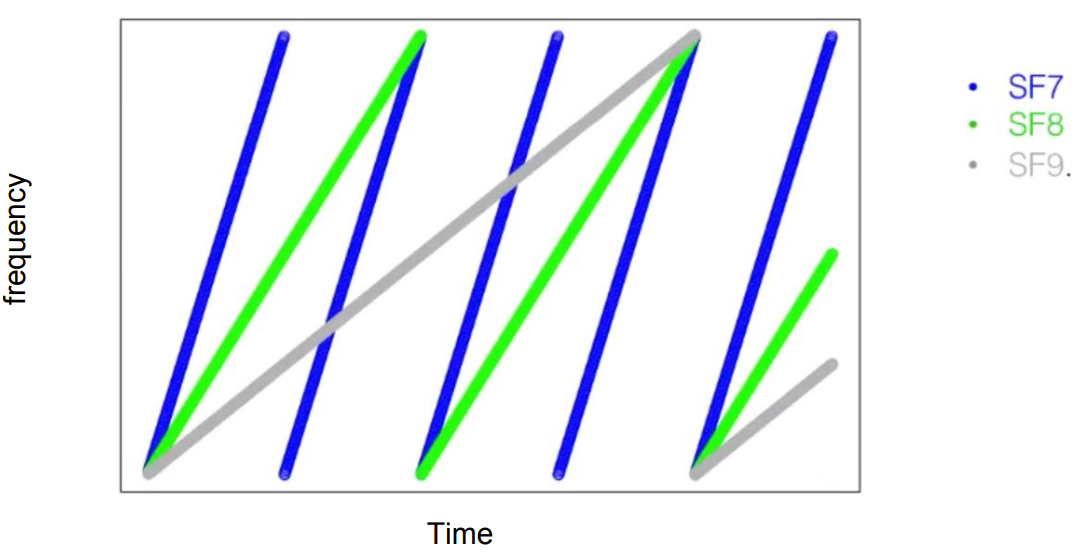
\includegraphics[width=0.6\textwidth]{Figures/spreading factors.png}
	\caption{Chirp signál a porovnanie rozprestieracích faktorov. Prevzaté z \cite{spreadfactorimage}}
	\label{fig:spreadingfactors}
\end{figure}

Existujú dva druhy chirp signálov, sú nimi up-chirp signál a down-chirp signál. Pri up-chirp signále sa prechádza zo spodnej hranice frekvenčného pásma do hornej hranice a pri 
down-chirp zase naopak.

\newpage
Ako rýchlo sa chirp posúva po frekvenčnom pásme - tzn. ako rýchlo chirp signál mení svoju frekvenciu, je určené parametrom rozprestierací faktor -- spreading factor (SF). 
Rozprestierací faktor zároveň vyjadruje, koľko bitov informácie je v každom symbole prenesených. Pri nižšom rozprestieracom faktore sa chirp signál posúva po 
frekvenčnom pásme rýchlejšie (viď Obr. \ref{fig:spreadingfactors}) a tým sa zvyšuje rýchlosť dátového prenosu, 
avšak zhoršuje sa citlivosť, ktorou dokáže prijímač prijať signál a dôsledkom toho je menší použiteľný dosah.

Každý chirp signál je rozdelený na X častí -- tzv. chips. Tieto chips predstavujú skoky vo vysielacej frekvencii signálu. 
Koľko týchto chips jeden chirp obsahuje je závisle od vybraného rozprestieracieho faktoru. 
Jeden chirp je rozdelený na $2^{SF}$ častí alebo chips.

Vysielaný symbol sa potom skladá z cyklicky posunutého chirp signálu, kde posun definuje hodnotu daného symbolu. 
To znamená, že vysielaný chirp nebude začínať na spodnej hranici frekvenčného pásma, ale na určitej frekvencii korešpondujúcej so symbolom, 
ktorý je modulovaný do daného chirp signálu. Viď Obr. \ref{fig:loraSymbols}.

\begin{figure}
	\centering
	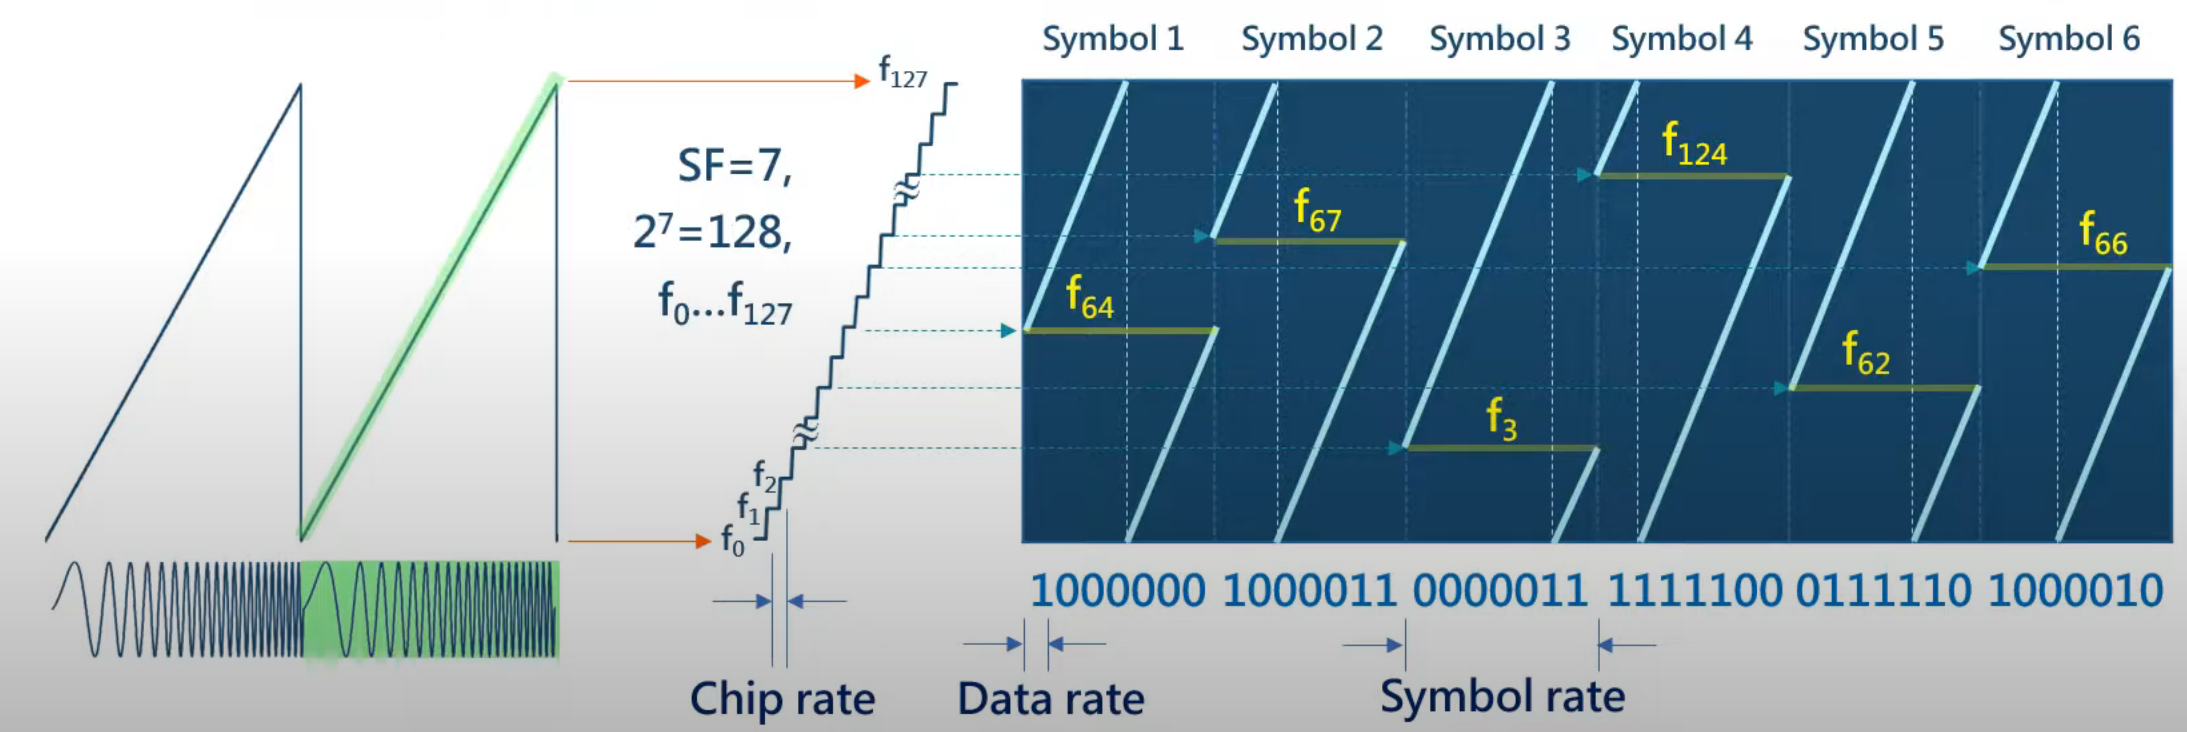
\includegraphics[width=1\textwidth]{Figures/loraSymbols.png}
	\caption{Chirp signály, do ktorých boli modulované symboly. Prevzaté z TODO}
	\label{fig:loraSymbols}
\end{figure}

Celý proces vyslania správy cez LoRa sa teda skladá z nasledujúcich krokov:
\begin{enumerate}
  \item Konverzia správy do binárneho kódu
  \item Pridanie korekčných bitov slúžiacich na opravu chýb
  \item Pridanie preambuly a kontrolného súčtu, a poskladanie do LoRa paketu
  \item Modulácia bitov do chirp signálov
  \item Odvysielanie chirp signálov
\end{enumerate}
Ukážku môžme vidieť na Obr. \ref{fig:loraModulation}.

\begin{figure}
	\centering
	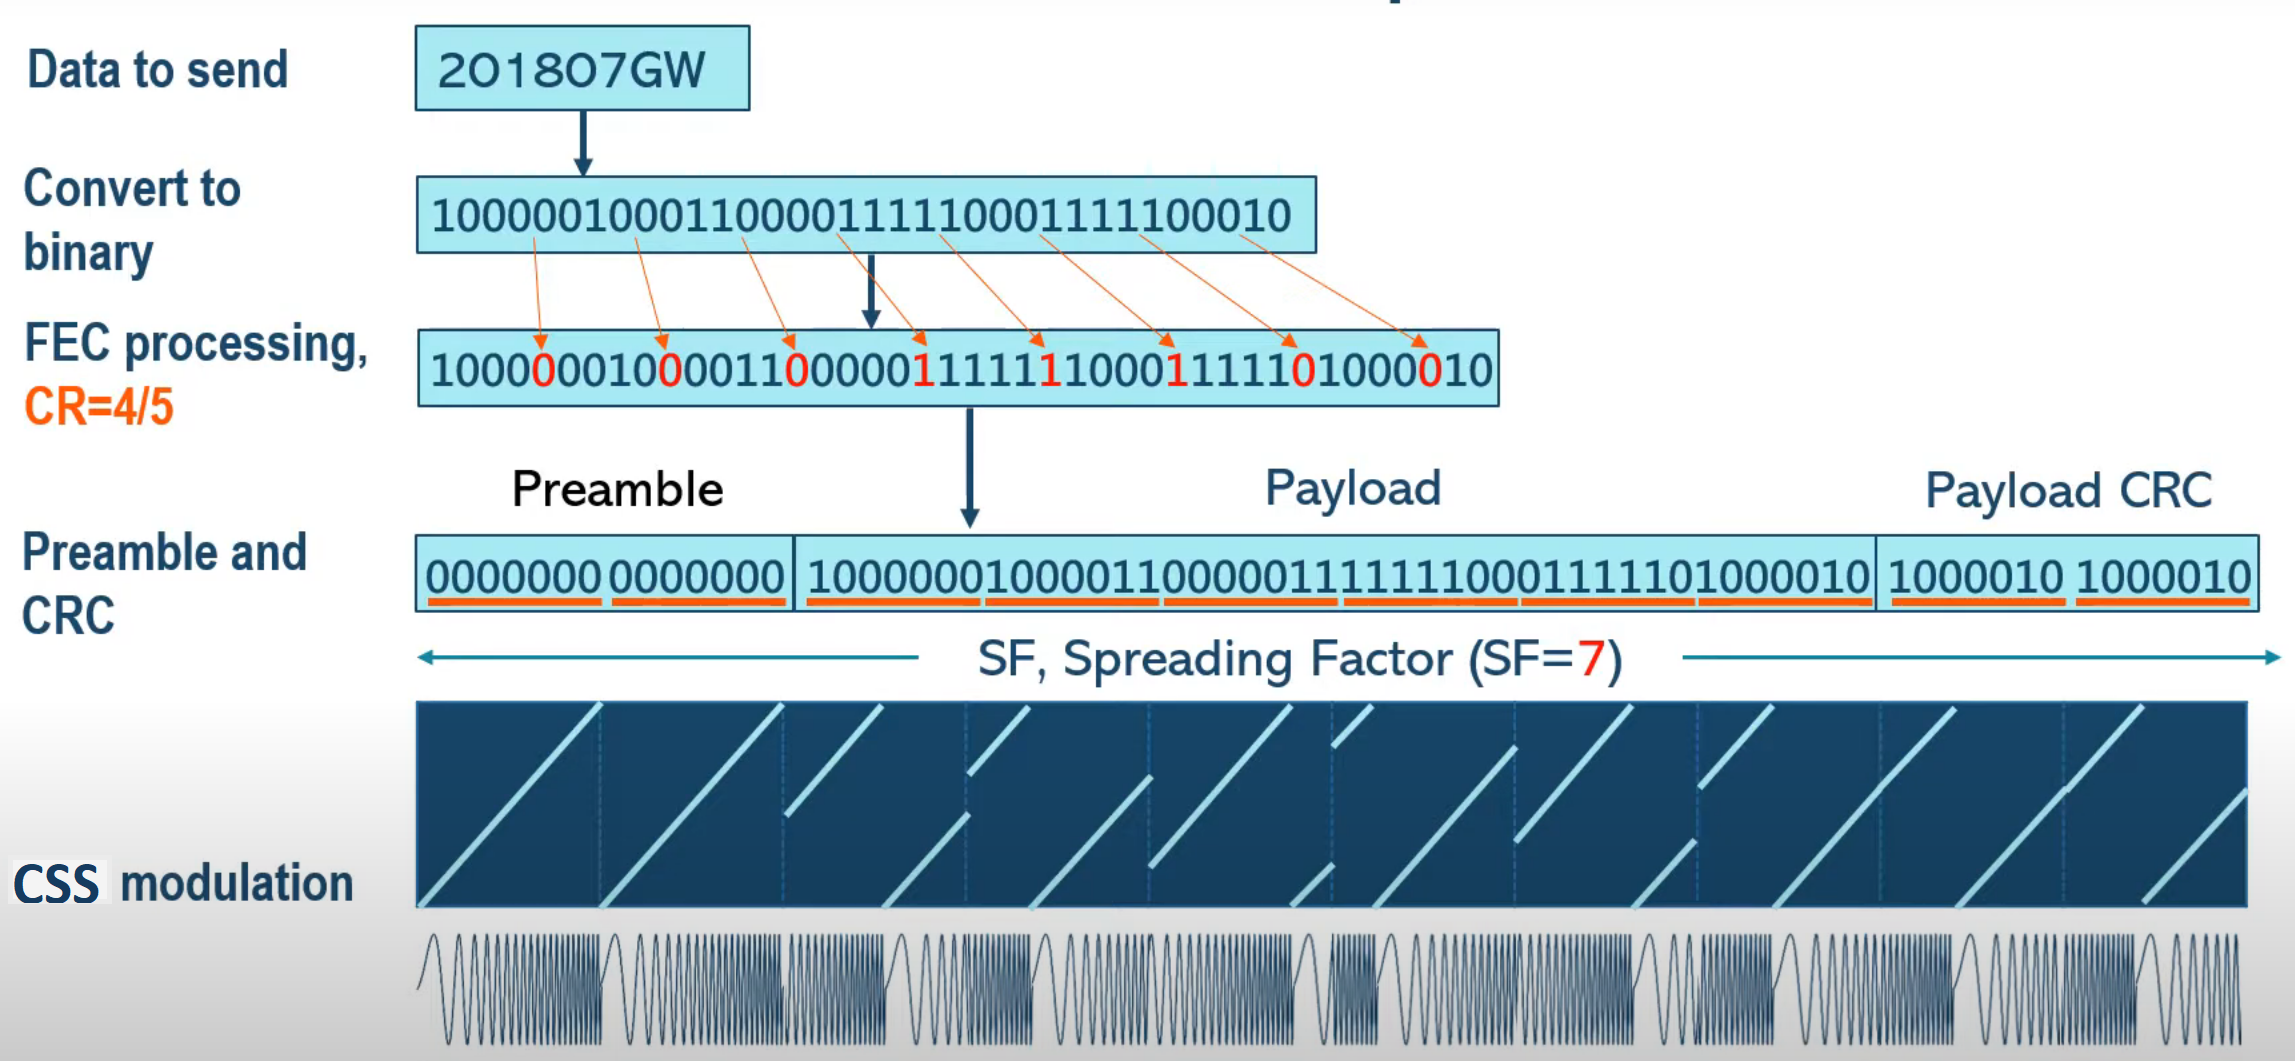
\includegraphics[width=1\textwidth]{Figures/loraModulation2.png}
	\caption{Proces spracovania odosielaných dát v LoRa (Binárne hodnoty su ukážkové, nezodpovedajú reálnej konverzií). Prevzaté z TODO}
	\label{fig:loraModulation}
\end{figure}

\section{LoRa paket}
Štruktúra LoRa paketu môže byť závislá od daného použitia. Bežné sa ale stretávame s LoRa paketom, zloženým z preambuly, dát a kontrolného súčtu.

Preambula slúži na synchronizáciu prijímacieho zariadenia. Je tvorená niekoľkými opakovaniami prázdneho chirp signálu, ktorý predstavuje symbol s hodnotou 0. 
Dĺžka preambuly, tzn. počet opakovaní prázdneho chirp signálu, je stanovená konfiguráciou zariadenia. Bežne sa stretávame s dĺžkou preambuly 8.
Na Obr. \ref{fig:loraModulation} môžme vidieť, že na preambulu boli použité iba 2 prázdne chirp signály -- teda dĺžka preambuly je 2.

Prijímacie zariadenie číta prijaté symboly v určitom časovom intervale -- okne. Tento interval sa ale nemusí zhodovať s intervalom, ktorý bol použitý pri vysielaní daných symbolov.
Je preto potreba synchronizovať prijímacie zariadenie aby hodnoty symbolov boli správne interpretované.

Zariadenie po prijatí nového paketu očakáva, že na začiatku bude preambula definovanej dĺžky. Ak z paketu prečíta počet symbolov rovnakej hodnoty, zhodný 
s definovanou dĺžkou preambuly, predpokladá že sa jedná o preambulu a synchronizuje čítacie okno tak aby bolo zarovnané so symbolmi preambuly. Tzn. tak, aby symboly preambuly boli 
prečítané ako symbol 0. 

Zjednodušené znázornenie procesu čítania symbolov a posun čítacieho okna môžme vidieť na Obr. \ref{fig:loraPreamble1}.

\begin{figure}[h!]
	\centering
	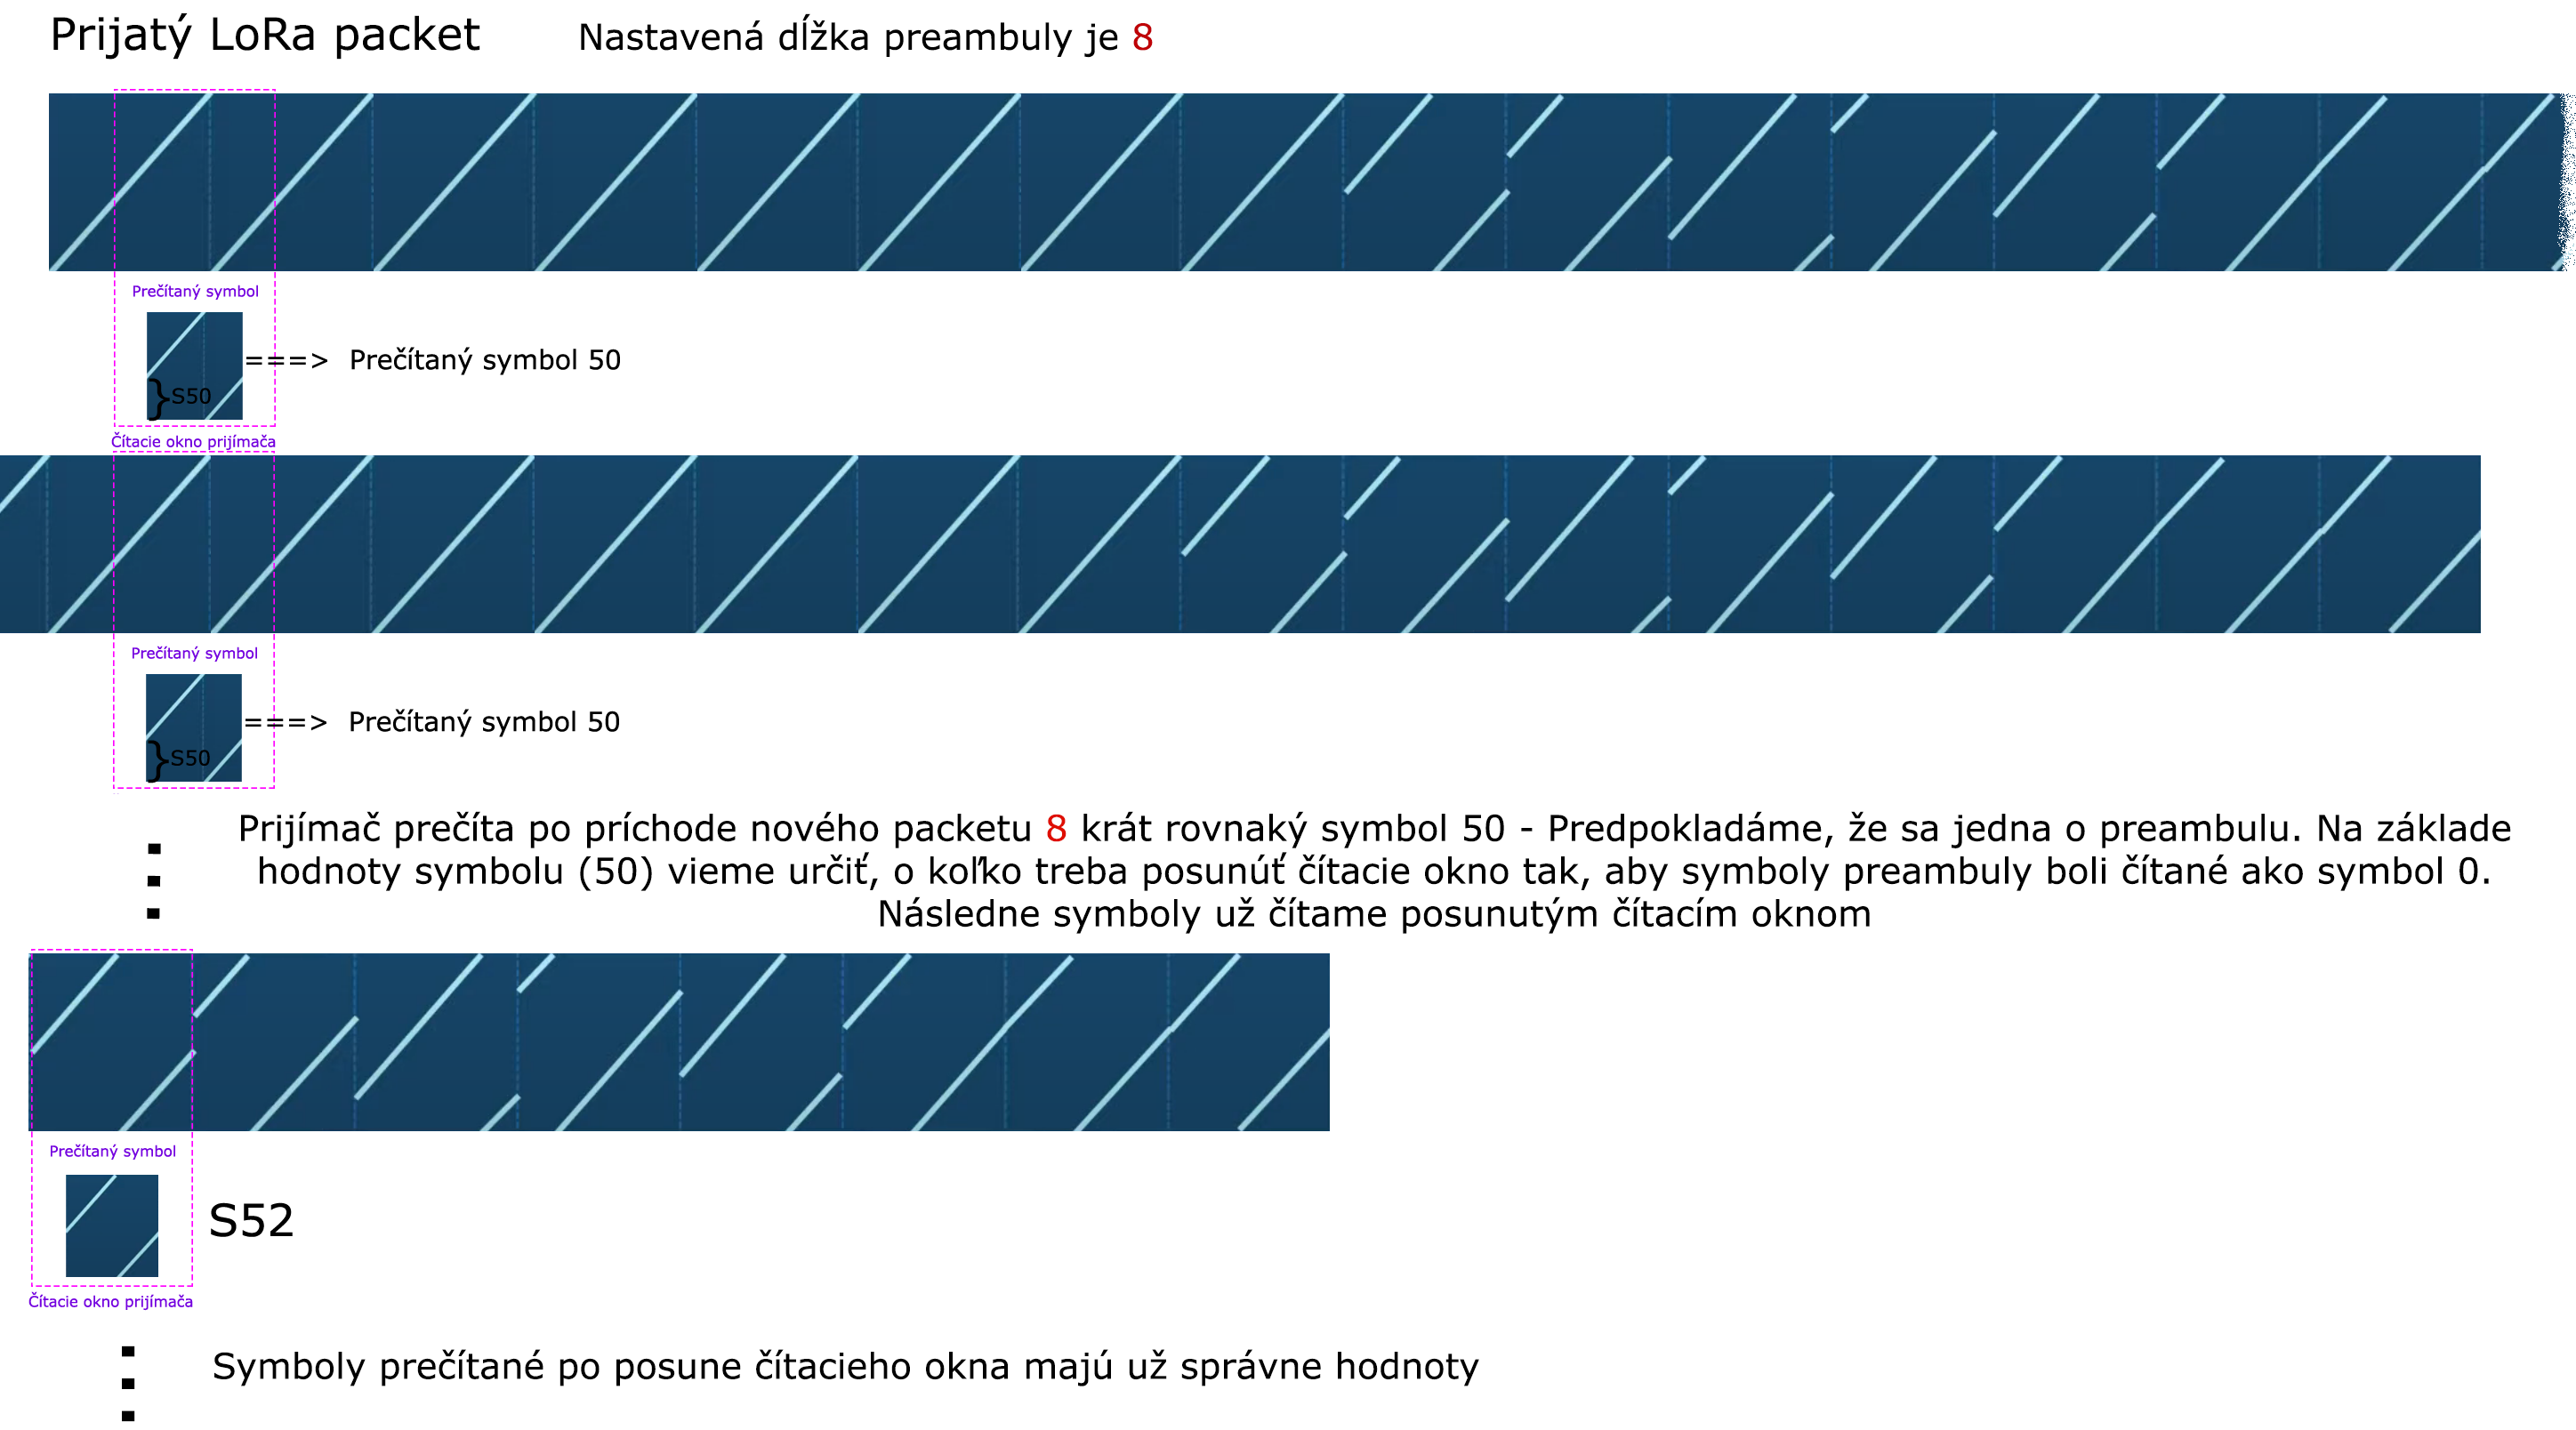
\includegraphics[width=1\textwidth]{Figures/preambulaSmall.png}
	\caption{Čítanie symbolov preambuly prijatého paketu a synchronizácia čítacieho okna na základe posunu preambuly.}
	\label{fig:loraPreamble1}
\end{figure}

\newpage
\section{LoRa parametre}
Pri používaní technológie LoRa je nutné správne zvoliť parametre na bezdrôtový prenos. Medzi nastaviteľné parametre patrí frekvencia, šírka pásma, rozprestierací factor a kódovací pomer.
Použitá frekvencia je závislá od regiónu, v ktorom chceme technológiu LoRa využívať, viď Tabuľka \ref{tab:ismBands}. 

V Európe je možné mimo 866 MHz pásma používať na LoRa aj 433 MHz pásmo. Okrem toho existuje ešte globálne používaná frekvencia 2,4 GHz. Tu sme ale limitovaní 
podporou daných frekvencií v nami použitom LoRa modeme. Bežné používané moduly, zväčša nemajú podporu pre 2,4 GHz frekvenčné pásmo.

\begin{table}[h!]
	\centering
  \small
  \setlength\tabcolsep{6pt}
	\caption[Frekvenčne pásma používane pre LoRa]{Frekvenčne pásma používane pre LoRa}
  \begin{tabular}{c|c}
    \toprule
    Región & Frekvenčné pásmo (MHz)\\
    \midrule
    Ázia & 433 \\
    Európa, Rusko, India, Afrika & 863--870 \\
    Severná Amerika & 902--928 \\
    Austrália & 915--928 \\
    Kanada & 779--787 \\
    Čína & 779--787, 470--510 \\
    \midrule
  \end{tabular}
  \label{tab:ismBands}
\end{table}
\newpage

Ostatné LoRa parametre sú vyberané na základe toho ako ďaleko, ako spoľahlivo a ako rýchlo je potrebné dáta prenášať. Je nutné zvoliť vhodný kompromis medzi rýchlosťou prenosu 
a dosahom prenosu.

Parameter bandwidth (BW) určuje šírku pásma, v ktorom sa bude chirp posúvať. Pri vyššej šírke pásma sa zvyšuje rýchlosť prenosu, avšak znižuje sa použiteľný dosah.
Najbežnejšie používané su šírky pásma 125 kHz, 250 kHz a 500 kHz.

Rozprestierací faktor -- spreading factor (SF) určuje koľko bitov dát bude prenesených v každom vysielanom symbole. To určuje ako rýchlo sa chirp posúva po frekvenčnom pásme a tym pádom 
zvyšuje alebo znižuje rýchlosť prenosu na úkor zníženia alebo zvýšenia dosahu prenosu. Spreading factor je vo väčšine prípadov možné zvoliť z intervalu 6--12. 
Avšak niektoré LoRa modemy umožňujú nastaviť aj nižšie hodnoty rozprestieracieho faktoru. 

Používanie rozprestieracích faktorov prináša výhodu v podobe ortogonality správ vysielaných s rôznymi rozprestieracími faktormi. 
To znamená, že prijímač dokáže správne prijať a dekódovať správu poslanú s rozprestieracím faktorom X aj 
keď sa vysielaná správa časovo prekrýva s inou vysielanou správou s iným rozprestieracím faktorom.

LoRa obsahuje korekciu chýb spôsobených rušením. Využíva k tomu samo-opravný kód -- forward error correction (FEC), pri ktorom 
sa ku prenášaným dátam pridávajú korekčné bity. Tieto bity sú potom na prijímacej strane použité na detekciu a prípadnú opravu chyby ak k nejakej došlo vplyvom rušenia.
K nastaveniu korekcie chýb slúži parameter kódovací pomer -- coding rate (CR).

V technológií LoRa máme na výber zo štyroch možností pre parameter coding rate: 4/5, 4/6, 4/7 a 4/8. 
Označenie vyjadruje pomer bitov, ktoré nesú informáciu, ku bitom, ktoré budú reálne použité na prenos informácie. 
Napríklad pri kódovacom pomere 4/5 sa na každé 4 bity informácie pridáva 1 korekčný bit.
Vyšší kódovací pomer zabezpečí spoľahlivejší prenos dát ak sa nachádzame v rušivom prostredí, avšak zníži rýchlosť prenosu dát, 
pretože ku prenášaným dátam pridáva navyše dáta potrebné na korekciu chýb.

Rýchlosť prenosu dát (Data rate -- DR) môžme vyjadriť vzťahom:
\begin{figure}[h!]
  \centering
  \[DR = SF * \frac{\frac{4}{4+CR}}{\frac{2^{SF}}{BW}} *1000 \]
  \begin{tabular}{c c}
    DR & rýchlosť prenosu dát v bitoch za sekundu\\
    BW & šírka pásma v kHz \\
    SF & rozprestierací faktor (hodnoty 6--12) \\
    CR & kódovací pomer (hodnoty 1--4) \\
  \end{tabular}
\end{figure}

\section{LoRaWAN}
Technológia LoRa je definovaná len na fyzickej vrstve. Na používanie LoRa v IoT sieťach sú však potrebné aj vyššie vrstvy sieťového modelu.
K tomu vznikol protokol LoRaWAN, ktorý je spravovaný organizáciou LoRa Alliance \cite{lora}.

LoRaWAN definuje komunikačný protokol a architektúru sieti. Siete používajú hviezdicovú topológiu, prípadne topológiu hviezdu hviezd, kde 
centrálnym uzlom je LoRaWAN brána -- gateway, ktorá je pripojená k internetu a pevnému napájaniu. Ostatne uzly siete posielajú dáta do tejto brány, 
ktorá ich potom preposiela na internet. Tam su už dáta dostupné odkiaľkoľvek.

LoRaWAN definuje tri základne triedy zariadení, ktoré sa v sieti vyskytujú. Triedy špecifikujú funkciu zariadenia a jeho vlastnosti.
Sú nimi triedy A, B a C, kde do triedy A spadajú zariadenia väčšinou poháňané batériami, ktoré po odvysielaní svojich dát otvárajú dve prijímacie okna, 
v ktorých čakajú na príjem dát z brány.
Trieda B je rozšírením triedy A. Zariadenia v tejto triede môžu otvárať dodatočné prijímacie okna v naplánovaných časových intervaloch.
Zariadenia z triedy C môžu prijímať neustále. Z tohto dôvodu majú vyššiu spotrebu energie a zvyčajne su pripojené k stálemu napájaniu.
TODO tu este zo tri styri  vety aby strana nekoncila prazdnym miestom

\section{Legislatíva}
V Európe sa k frekvenčnému pásmu používaného v technológií LoRa viažu určité obmedzenia. 
Obmedzenia sa týkajú používania fyzického média. Regulácia určuje maximálnu povolenú dobu, v ktorú môže vysielač na daných frekvenciách vysielať 
v rámci jednej hodiny a maximálny vysielací výkon, akým môže signal vysielať.

Určuje sa takzvaný klučovací pomer, ktorý hovorí koľko percent času z nejakého celkového času môže vysielač vysielať.
Ak by zariadenie vysielalo signál po dobu jednej jednotky času z celkových 10 jednotiek času, tak kľučovací pomer by bol 10 \%.

Český Telekomunikačný úrad \cite{ctu} stanovuje vo všeobecné oprávnění č. VO-R/10/07.2021-8 \cite{vor}, že 
frekvenčné pásmo, do ktorého spadá technológia LoRa, patrí do skupiny g. Pre túto skupinu je maximálny povolený kľučovací pomer 1 \% a maximálny 
vysielací výkon 25 mW (14 dBm). Znamená to teda, že zariadenia môžu každú hodinu vysielať maximálne po dobu 36 sekúnd.
Pre pásmo 869,40--869,65 MHz je ale udelená výnimka, ktorá umožňuje vysielať s kľučovacím pomerom 10 \% a maximálnym vysielacím výkonom 500 mW (27 dBm).

\chapter{Dostupné LoRa moduly }
Pri práci s technológiou LoRa máme na výber z rôznych modulov od rôznych výrobcov.
Moduly môžme rozdeliť podla použitia na moduly pre koncové zariadenia a moduly pre gateway.
Moduly pre koncové zariadenia obvykle dokážu prijímať a odosielať iba na jednom kanále ( kombinácia LoRa parametrov --  BW, SF, CR a frekvencia ) súčasne a majú 
nízku spotrebu energie. Moduly pre gateway dokážu prijímať a odosielať na viacerých kanáloch súčasne ale majú vyššiu spotrebu energie.

V tejto časti sa budeme zaoberať dostupnými modulmi pre koncové zariadenia.
Keďže je technológia LoRa patentovaná výrobcom Semtech \cite{semtech}, tak všetky dostupné LoRa čipy su práve od tohto výrobcu a moduly od iných výrobcov 
sú založené na používaní týchto čipov.

\section{SX127x/SX126x}
Výrobca Semtech \cite{semtech}, prináša LoRa čipy série SX127x a SX126x. Ponúkajú vysoký výkon za pomerne nízku cenu a ako sme už spomínali, ostatné LoRa moduly 
iba implementujú tieto LoRa čipy -- modemy a rozširujú ich o ďalšiu funkcionalitu.

\subsection{SX127x}
SX127x LoRa modemy používajú LoRa modulačnú techniku frequency hopping spread-spectrum, patentovanú firmou Semtech.

Maximálny vysielací výkon týchto modemov je 100 mW.
Vďaka použitej modulačnej technike je možné dosiahnuť vysokej citlivosti modemov.
Výrobca uvádza citlivosť cez -137 dBm pri modemoch SX1272/73 a -148 dBm pri modemoch SX1276/78/79.

%TODO vysvetlivka linkbudget do footnote
Modemy SX1272 a SX1273 ponúkajú menší link budget 157 dB oproti 168 dB pri modemoch SX1276/77/78/79 a majú menší rozsah frekvenčných pásiem medzi 860 a 1020 MHz.
Okrem toho majú aj vyššiu spotrebu energie.

Pri modemoch SX1276/77/78/79 je možné vybrať frekvenčné pásma z rozsahu 137 až 1020 MHz.

\subsection{SX126x}

Modemy zo série SX126x - SX1261/62/68 sú nasledovníkmi predošlých modemov SX127x. Majú väčší vysielací výkon vďaka integrovanému zosilňovaču a menšiu spotrebu energie. 
Obsahujú precízny TCXO oscilátor, ktorý zabezpečuje presnejšie a stabilnejšie riadenie počas prevádzky modemu. Okrem LoRa modulácie obsahujú aj G(FSK) moduláciu, ktorá je vhodná pre staršie 
prípady použitia.

Modemy obsahujú +22/+15 dBm zosilňovač, vďaka ktorému majú vyšší link budget oproti modemom zo série SX127x. 
Ten je pri modemoch série SX126x výrobcom udávaný na 170 dBm, takže sú optimálne pre aplikácie vyžadujúce väčší dosah alebo robustnosť.
%TODO este pripadne modem 1280/1281 - 2.4ghz

\begin{table}[!h]
	\centering
  \small
  \setlength\tabcolsep{6pt}
	\caption[Parametre Semtech SX modemov]{Parametre Semtech SX modemov}
  \begin{tabular}{c|c|c|c|c|c|c|c|c}
    \toprule
    Modem & Frekvencia & SF & BW (kHz) & Citlivosť & Spotreba \footnotemark[1] & Rozhranie & Výkon\footnotemark[2] & Cena\footnotemark[3]\\
    \midrule
    SX1272 & 860--1020 MHz & 6--12 & 125--500 & -137 dBm & 11,2 mA & SPI & 20 dbm & 9€ \\
    SX1273 & 860--1020 MHz & 6--9 & 125--500 & -130 dBm & 11,2 mA & SPI & 20 dbm & 7€ \\
    SX1276 & 137--1020 MHz & 6--12 & 7,8--500 & -148 dBm & 12 mA & SPI & 20 dbm & 10€ \\
    SX1277 & 137--1020 MHz & 6--9 & 7,8--500 & -139 dBm & 12 mA & SPI & 20 dbm & 7€ \\
    SX1278 & 137--525 MHz & 6--12 & 7,8--500 & -148 dBm & 12 mA & SPI & 20 dbm & 8€ \\
    SX1279 & 137--960 MHz & 6--12 & 7,8--500 & -148 dBm & 12 mA & SPI, UART & 20 dbm & 11€ \\
    \hline
    SX1261 & 150--690 MHz & 5--12 & 7,80--500 & -125 dBm & 8 mA & SPI & 15 dbm & 7€ \\
    SX1262 & 150--690 MHz & 5--12 & 7,80--500 & -125 dBm & 8 mA & SPI & 22 dbm & 8€ \\
    SX1268 & 410--810 MHz & 5--12 & 7,80--500 & -148 dBm & 4.6 mA & SPI & 22 dbm & 7€ \\
    \midrule
  \end{tabular}
\end{table}
\footnotetext[1]{Spotreba počas prijímania (mA)}
\footnotetext[2]{Maximálny vysielací výkon}
\footnotetext[3]{Cena platná ku Q4 2022}

\section{RFM9xW}
Moduly RFM95W/96W/98W od výrobcu HopeRF \cite{hoperf} implementujú SX LoRa modemy od výrobcu Semtech.
Jedná sa o jednoduchý modul, ktorý obsahuje všetku riadiacu elektroniku potrebnú pre riadenie Semtech LoRa modemu.
Okrem riadiacej elektroniky obsahuje modul aj zosilňovač signálu (+14 dBm), ktorý zvyšuje dosah bezdrôtového prenosu.

Existuje niekoľko verzií modulov RFM9xW, kde každá verzia používa iný semtech LoRa modem a zdieľa parametre daného modemu.

\section{Moduly a zariadenia použité v tejto práci}
Na vývoj a testovanie tejto práce boli použité rôzne zariadenia s rôznymi platformami. Na simulovanie jednoduchých koncových zariadení, 
ktoré môžu predstavovať napríklad nejaký senzor, boli použité mikrokontroléry TTGO od výrobcu LILYGO \cite{lilygo}.

Okrem mikrokontrolérov TTGO boli použité aj mikrokontroléry Raspberry Pi Pico a jednodoskový počítač Raspberry Pi.
Nami použité mikrokontroléry môžu byť neskôr rozšírene o batériu a byť mobilné.

\subsection{TTGO LoRa32}
Tento mikrokontrolér je založený na module ESP32. Obsahuje Wi-Fi, bluetooth a LoRa moduly. 
Konkrétne používa SX1276 LoRa modem.

Dá sa prepnúť do úsporného režimu spánku, ktorý znižuje spotrebu mikrokontroléru na 0,6 mA.
Mikrokontrolér obsahuje aj 0,96 palcový čiernobiely displej, ktorý je pripojený cez I2C rozhranie.

\subsection{TTGO T-Beam}
Tento mikrokontrolér je taktiež založený na module ESP32 a obsahuje Wi-Fi, bluetooth a LoRa modul.
Rovnako používa SX1276 LoRa modem no okrem spomínaných modulov obsahuje aj GPS modul.

Mikrokontrolér ma na zadnej strane držiak na batériu, z ktorej môže byť napájaný a taktiež aj nabíjací modul 
pre bezpečné nabíjanie a ochranu lítiových batérií.
V režime spánku ma spotrebu 0,2 mA.

Podporuje pripojenie dodatočného displeju, avšak nami používaný mikrokontrolér tento displej nemá.

Na Obr \ref{fig:ttgo-moduly} môžeme vidieť oba mikrokontroléry TTGO.
\begin{figure}[h!]
  \centering
  \subfloat[\centering TTGO LoRa32]{{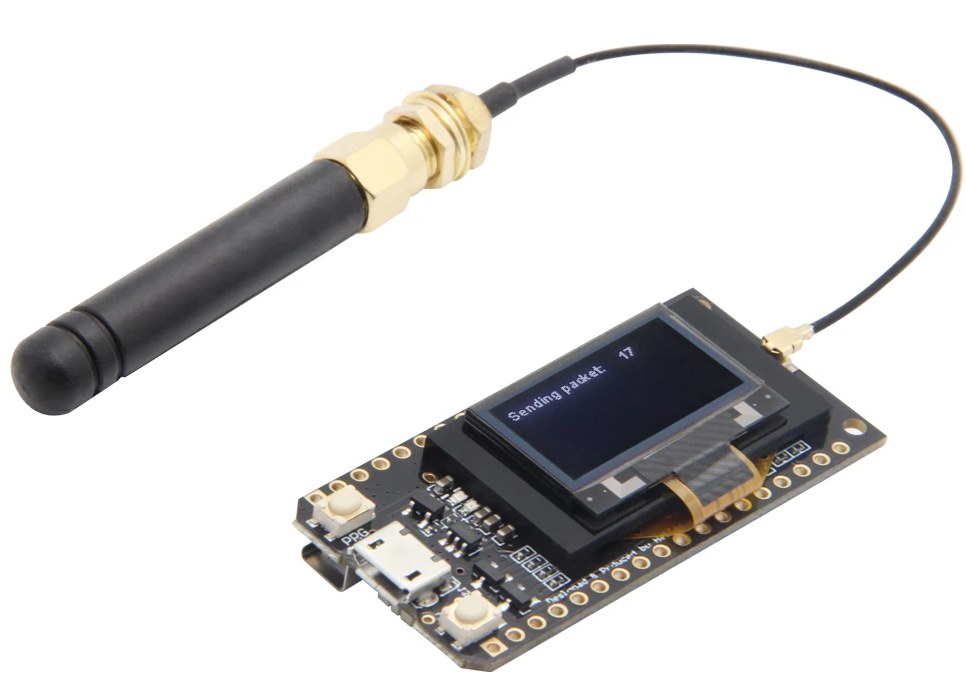
\includegraphics[width=0.4\textwidth]{Figures/LILYGO-TTGO-LoRa32-V1.png} }}
  \qquad
  \subfloat[\centering TTGO T-beam]{{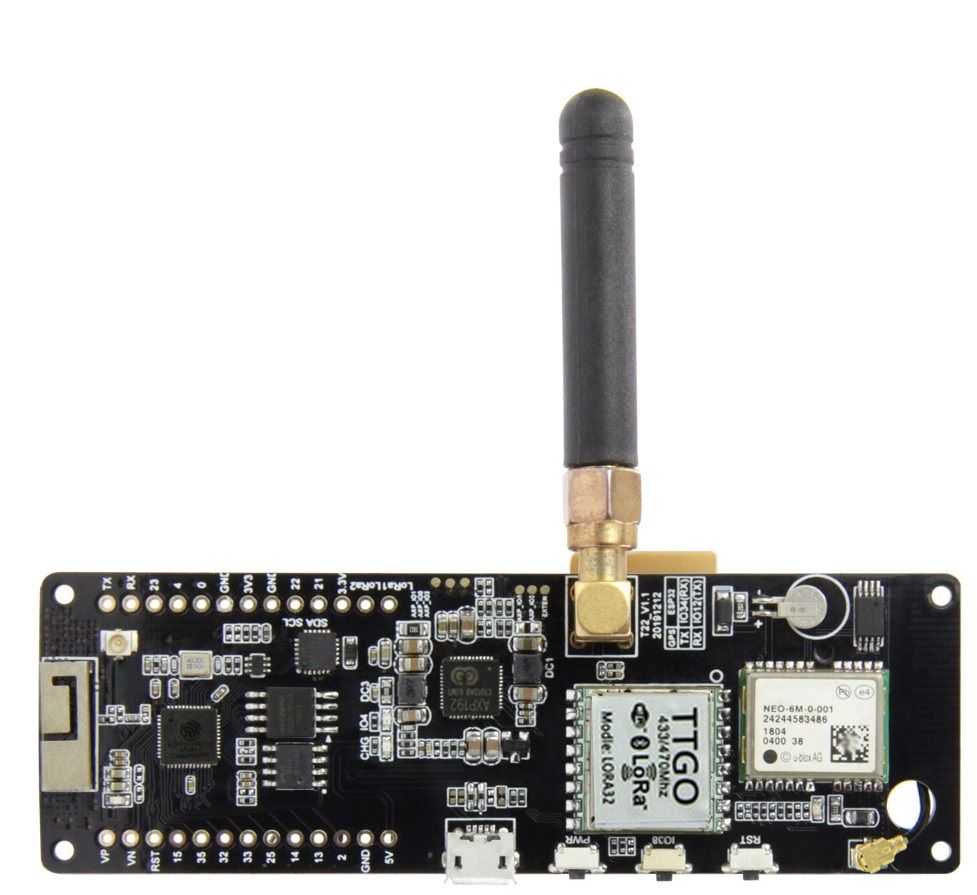
\includegraphics[width=0.35\textwidth]{Figures/ttgo-tbeam.jpg} }}
  \caption{Mikrokontroléry TTGO}
  \label{fig:ttgo-moduly}
\end{figure}

\subsection{Raspberry Pi Pico RP2040}
Mikrokontrolér od známej organizácie Raspberry Pi, založený na dvoj-jadrovom Arm procesore. 
Existuje verzia s Wi-Fi modulom aj bez. Na programovanie sa využíva jazyk C alebo MicroPython, 
prípadne derivát MicroPythonu -- CircuitPython. V tejto práci bude použitý práve CircuitPython.

Avšak aby bolo možné využívať tieto mikrokontroléry s technológiou LoRa, bolo potrebné pridať k nim nejaký LoRa modul.

%TODO armachat footnote?
Na implementáciu v tejto práci boli preto zvolené zariadenia Armachat, ktoré kombinujú mikrokontrolér Raspberry Pi Pico s LoRa modulom RFM96W.
Okrem toho pridávajú dvoj palcový farebný displej a klávesnicu.

Ako toto zariadenie vyzerá môžme vidieť na Obr \ref{fig:armachat}.

\begin{figure}[h!]
	\centering
	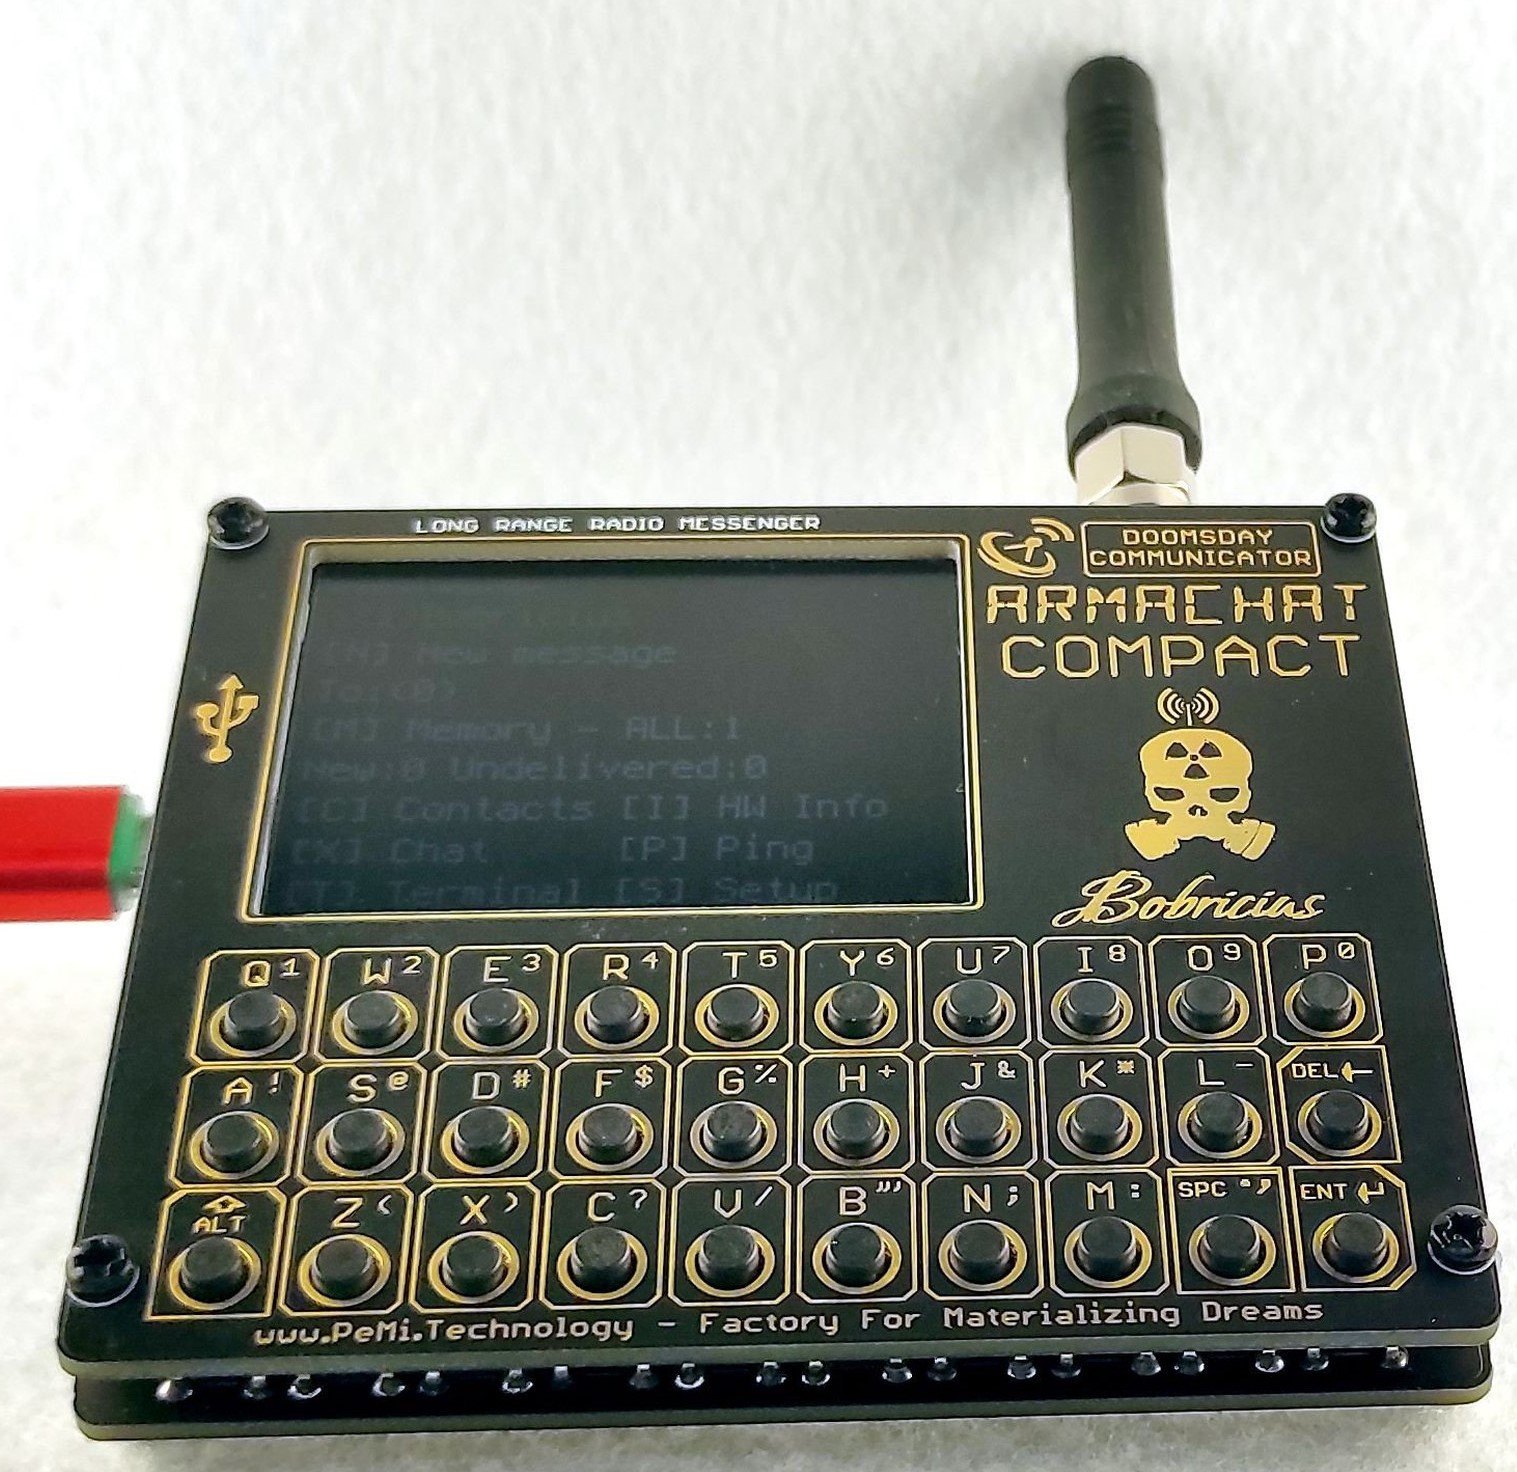
\includegraphics[width=0.4\textwidth]{Figures/armachat.jpg}
	\caption{Zariadenie Armachat}
	\label{fig:armachat}
\end{figure}

\subsection{Raspberry Pi 2B}
Jednodoskový štvor-jadrový počítač vytvorený organizáciou Raspberry Pi.

Zariadenie obsahuje eternetový port, ktorý môže slúžiť na pevné pripojenie do internetovej siete.
Počítač sam o sebe neobsahuje žiaden modul a tak pre prácu s LoRa bude pridaný RFM96W modul pripojený do vstupno-výstupných pinov počítača.

Na rozdiel od predchádzajúcich mikrokontrolérov disponuje tento jednodoskový počítač oveľa väčším výkonom a pamäťou, 
avšak ma oveľa vyššiu spotrebu energie. Z tohto dôvodu bude tento počítač plniť rolu nemobilného uzlu v sieti, ktorý bude pripojený cez ethernet do internetovej siete.

Vďaka tomu, že CircuitPython je možne spojazdniť aj na Raspberry Pi, bude možné čast implementácie zdielať medzi Raspberry Pi Pico a Raspberry Pi 2B.


\chapter{Existujúce riešenia}
Téma mesh sietí je v tejto dobe veľmi aktuálna a vývojári sa snažia vytvoriť rôzne riešenia, ktoré by boli vhodné pre rôzne účely.
Existujú rozvinuté projekty ako napríklad Meshtastic, ktorý sa snaží vytvoriť rozsiahlu decentralizovanú mesh sieť za použitia lacných zariadení.

Ďalším zaujímavým projektom je Armachat \cite{armachat}, ktorý ponúka možnosť komunikácie v prípade nedostupnosti ostatných sieti, napríklad po nejakej prírodnej alebo inej katastrofe.
Súčasťou projektu Armachat sú plošné spoje, z ktorých si používateľ poskladá finálne zariadenie.
Zariadenia Armachat su poháňané mikrokontrolérmi Raspberry Pi Pico, obsahujú LoRa moduly, displej, klávesnicu a ďalšie vymoženosti.

Originálny projekt avšak sám o sebe nepodporuje využívanie mesh topológie. Používa ale rovnakú štruktúru správ ako projekt Meshtastic a vďaka tomu je možné 
v projekte Armachat využívať mesh sieť projektu Meshtastic.

\section{LoRa mesher}
LoRaMesher \cite{loramesher} je knižnica, ktorú je možné použiť na komunikáciu v LoRa mesh sieti.

Na smerovanie v sieti sa používa distance vector routing protokol. Tento protokol vyberá cestu, kadiaľ bude správa v sieti preposlaná od odosielateľa k príjemcovi, na základe 
najlepšej cesty. Najlepšiu cestu definuje ako cestu s najmenším počtom hopov -- preskokov medzi uzlami v mesh sieti.

K realizácií distance vector smerovania je potrebné udržiavať smerovaciu tabuľku, ktorá obsahuje informácie o ID uzlov, cez ktoré susedné uzly sa dané uzly dajú dosiahnuť a 
koľko preskokov bude potrebných na dosiahnutie týchto uzlov. Smerovacia tabuľka je periodicky aktualizovaná cez špeciálny typ správ, ktoré sú odosielané 
všetkými uzlami v sieti. Túto smerovaciu tabuľku si drží a priebežne aktualizuje každý uzol v sieti.

LoRaMesher používa FreeRTOS, čo je operačný systém reálneho času. Takéto operačné systémy garantujú dokončenie úloh v určitom čase.
FreeRTOS je použitý na zabezpečenie plánovania úloh. Rozličné úlohy sa starajú o prijatie a odoslanie paketov, iné úlohy sa starajú o samotne 
spracovanie prijatých paketov.

LoRaMesher dokáže nájsť novo vytvorené uzly v sieti vďaka smerovaciemu protokolu. Pri odoslaní správ čaká na prijatie potvrdzujúcej -- ACK správy, ktorá potvrdzuje, 
že správa bola prijatá a tým zaisťuje spoľahlivosť. Správy väčšie ako 222 bajtov rozdeľuje na viacero správ, ktoré pošle postupne.

\section{Meshtastic}
Meshtastic \cite{meshtastic} vytvára mesh sieť za použitia lacných mikrokontrolérov s LoRa modulmi.
Myšlienka tohto projektu spočíva v tom, že vytvára komunikačnú sieť na miestach kde neexistuje spoľahlivá infraštruktúra na bezdrôtovú komunikáciu (napr. v horách).

Posielanie správ v sieti je založené na jednoduchom multi-hop flooding.
Každý uzol znovu odvysiela paket, ktorý prijal ( pokiaľ nedošiel počet preskokov na 0 ), až kým sa paket nedostane do určenej destinácie naprieč mesh sieťou.
Prenášane správy su šifrované za pomoci šifrovacieho algoritmu AES.

Zariadenia používane v projekte Meshtastic majú okrem LoRa modulu zabudovaný aj bluetooth modul, vďaka ktorému je možne sa k zariadeniu pripojiť cez mobilný telefón, ktorý slúži ako rozhranie pre 
užívateľa. Cez aplikáciu v mobilnom telefóne môže používateľ vytvárať a prijímať správy. Správy sa cez bluetooth prenášajú z telefónu do zariadenia kde sa následne odošlú cez 
LoRa do siete.

Meshtastic poskytuje možnosť pripojenia sa k oficiálnemu meshtastic mqtt brokerovi. Toto umožňuje prepojiť malé lokálne mesh siete do väčšej globálnej siete a 
tak rozšíriť dosah siete.

\section{LoRaBlink}
Ďalší multi-hop protokol, ktorý požíva časovú synchronizáciu medzi uzlami. Časová synchronizácia definuje sloty, v ktorých môže uzol pristupovať ku prenosovému médiu a 
vysielať svoje dáta. Správy sa sieťou šíria pomocou multi-hop flooding.

Sieť sa skladá z jedného uzlu, ktorý plní rolu takzvaného datasinku (gateway alebo brána) a ostatných uzlov. Uzly siete posielajú dáta do datasinku alebo data z neho prijímajú.

V určitých intervaloch datasink vyšle tzv. beacon signál. Tento signál slúži na časovú synchronizáciu medzi uzlami a značí začiatok novej epochy. 
Každá epocha obsahuje N slotov, v ktorých môžu uzly vysielať data. Beacon správa obsahuje hop count, ktorá udáva vzdialenosť ku datasinku.
Ked nejaký uzol príjme beacon signál, vyšle svoj vlastný beacon signál v ďalšom volnom slote, ktorý vyberá na základe vzdialenosti od datasinku (hop count).

Ked uzol potrebuje poslať nejaké dáta, tak vyberie najskorší volný slot a v nom vysiela svoje dáta. Ak tieto dáta príjme uzol, ktorý nie je datasink a 
hop count daného uzlu ku sinku je menší ako hop count vysielacieho uzlu, tak dáta v ďalšom volnom slote znovu prepošle. Toto sa opakuje, až 
kým data nedosiahnu datasink.

Takto tvorená sieť avšak vyžaduje existenciu nejakého hlavného uzlu (datasinku), ktorý je potrebný na riadenie siete prostredníctvom časovej synchronizácie.

\section{Pymesh}
Pymesh je súčasťou Pycom \cite{pycom} ekosystému. Tento ekosystém je určený na vývoj IoT systémov. Ponúka rôzne zariadenia, ktoré su určené na použitie s týmto 
ekosystémom. Zariadenia obsahujú WiFi, bluetooth a LoRa, prípadne SigFox moduly. Zariadenia je možné rozšíriť o rôzne moduly so senzormi, ktoré rozširujú ich schopnosti.

PyMesh sieť sa skladá z uzlov, ktoré môžu vystupovať v roli gateway alebo bežného uzla. Uzly typu gateway su označované ako Border Routers a prepájajú LoRa sieť s 
internetom. Uzly v sieti môžu komunikovať ad-hoc. V sieti môže dojsť k situácií kedy bude chcieť viacero uzlov vysielať v rovnakom čase a došlo by tak ku kolízií.
Aby sa zabránilo takýmto situáciám, je použitá metóda Listen Before Talk, pri ktorej sa pred vysielaním signálu overí, či nie je v sieti už niekto iný, kto by práve 
vysielal. Pokiaľ áno, tak sa posielaná správa vyšle neskôr.

PyMesh je primárne určený na použitie s Pycom zariadeniami a použitie na inom zariadení by vyžadovalo väčšie úpravy zdrojového kódu.

\section{Synchronous LoRa Mesh}
Tento projekt\cite{synchronouslorameshnetwork} vznikol z potreby získavania real-time dát z podzemných kanalizácií. Tieto dáta sú potrebné k monitorovaniu a predikcií kritických situácií akými 
sú napríklad záplavy.

LoRaWan však nemá moc veľký dosah do podzemia. Z toho dôvodu by bolo potrebné v podzemných priestoroch implementovať LoRaWan gateway-e, ktoré su ale energeticky náročne, drahé a vyžadujú 
pevné pripojenie do elektrickej a prípadne aj internetovej siete, ktoré v kanalizáciách niesu dostupné. Okrem toho, by museli byť všetky ostatné uzly v podzemnej sieti v dosahu danej gateway a pri väčšej podzemnej sieti 
by teda bolo potrebné implementovať viacero LoRaWan gateway.

Tento projekt sa snaží vyriešiť tieto problémy. Prináša protokol, ktorý rozširuje LoRaWan o tzv. repeater uzly (RN) viď Obr. \ref{fig:synchronouslora}. Tieto uzly sa vyskytujú na povrchu a preposielajú dáta z 
podzemných monitorovacích uzlov (sensor node  - SN) do LoRaWan siete. Monitorovacie uzly pod zemou tvoria mesh sieť a RN plní funkciu riadiaceho uzlu pre podzemnú mesh sieť. 
Komunikácia medzi RN a SN je synchronizovaná pomocou presného časovania, čo umožňuje koordináciu zmeny stavov SN z režimu spánku do normálneho režimu v čase, kedy 
potrebuje SN prijímať a odosielať dáta. Komunikácia sa cez uzly šíri multi-hop prístupom, za použitia smerovacej tabuľky.

Protokol používa na riadenie komunikácie metódu TDMA. RN priradí každej SN časový slot, v ktorom SN môže vyslať alebo prijať dáta.
Monitorovacie uzly su väčšinu času v režime spánku, zobudia sa len v ich určenom časovom slote a vďaka tomu majú tieto uzly nízku spotrebu energie.

Novo pripojený uzol do siete musí čakať na periodický beacon, vysielaný RN uzlom. Všetky uzly si držia v sebe smerovaciu tabuľku. Po pripojení nového uzla sa sieťou sa propaguje 
správa na aktualizovanie smerovacej tabuľky.

\begin{figure}
	\centering
	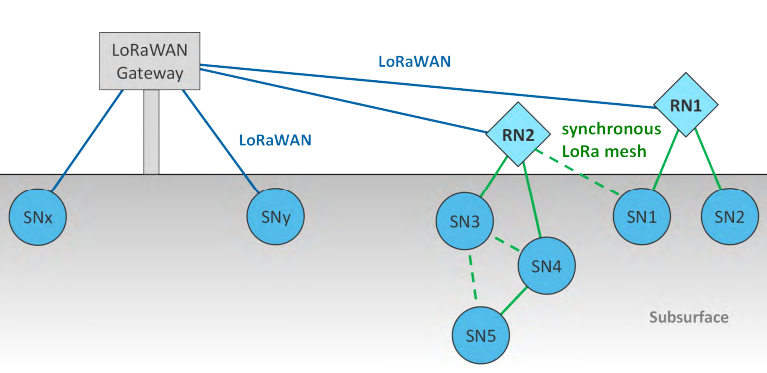
\includegraphics[width=0.6\textwidth]{Figures/synchronouslorameshnetwork.png}
	\caption{Schéma Synchronous LoRa Mesh. Prevzaté z \cite{synchronouslorameshnetwork}}
	\label{fig:synchronouslora}
\end{figure}

\section{Porovnanie voči nášmu riešeniu}
Niektoré zo spomenutých riešení využívajú smerovacie tabuľky na efektívnejší prenos dát v rámci siete. Smerovacie tabuľky môžu byť však limitáciou pokiaľ 
chceme dosiahnuť mobility uzlov. V prípade, že by sme chceli podporovať mobilitu uzlov, je potrebné zabezpečiť dostatočné časté aktualizácie smerovacích tabuliek.
To pridáva do siete zaťaženie v podobe dodatočných dátových prenosov.

Niektoré spomenuté riešenia limitujú komunikáciu medzi uzlami na vyhradené časové okná, mimo ktoré su uzly v úspornom režime. To môže byť 
veľkou limitáciou pri niektorých aplikáciách, kde je potrebná komunikácia v reálnom čase  (napr. chat).

Protokol navrhnutý v tejto práci nebude využívať žiadne smerovacie tabuľky. Vďaka tomu dosiahneme mobility uzlov bez potreby 
periodických aktualizácií smerovacích tabuliek. Hlavným využitím nášho protokolu je komunikácia v reálnom čase, preto protokol nebude používať 
žiadnu časovú synchronizáciu ani časové okná vyhradené na komunikáciu, uzly siete tak budu môcť prijímať a odosielať dáta hocikedy.
To so sebou ale prináša nevýhodu v podobe vyššej spotreby energie.

Funkcionalita navrhnutého protokolu bude, podobne ako niektoré zo spomínaných riešení, fungovať na základe multi hop flooding, kedy sa správa v sieti preposiela cez uzly siete až kým nedorazí do destinácie.
Správa sa odošle a uzol, ktorý túto správu prijal ako posledný ju prepošle ďalej. Toto sa opakuje na ostatných uzloch v sieti až kým sa správa nedostane do destinácie alebo kym správe nedôjde limit preskokov, prípade TTL.

Navrhnutý protokol nie je závislý na žiadnych špeciálnych centrálnych uzloch typu gateway, prípadne nejakých riadiacich uzloch. Každý uzol v sieti môže byť jednoduchým uzlom, ktorý bude prijímať a preposielať dáta ďalej.
Vďaka tomu môžu byť uzly realizované prostredníctvom lacných a malých zariadení.

Protokol bude možné používať na rôznych platformách. V tejto práci vznikne implementácia protokolu pre mikrokontroléry používajúce programovací jazyk C++ a 
mikrokontroléry alebo jednodoskové počítače podporujúce CircuitPython.

TODO nasa implementacia  je sifrovana AES

TODO tu by sa hodila tabulka s porovnanim (napr multiplatformovy support, spotreba energie, mobilita uzlov, obstaravacie naklady, zavislost na centralnych uzloch)

\chapter{Vlastná implementácia}
Ako sme už spomínali v predchádzajúcej kapitole, nami vytvorený protokol bude fungovať na základe multi hop flooding. Tento prístup so sebou ale nesie 
niekoľko nevýhod, ktoré by sme mali zohľadniť pri navrhovaní implementácie.

Jednou z nevýhod je, že ak pošleme niekam správu, a destinácia práve nie je v dosahu, tak by sme správu prišli. Tento problém vyriešime tak, 
že odosielateľ si bude odoslané správy ukladať a v prípade, že sa nepodarí správu doručiť, môže ju opätovne 
odoslať niekedy neskôr. To, že sa správu nepodarilo doručiť do destinácie, zistíme vďaka potvrdzovacím ACK správam. Tieto správy sa odosielajú v opačnom smere ako správa, ktorú potvrdzujeme. 

Ďalším z problémov môže byť potenciálne zahltenie siete správami. Keby každý uzol v sieti preposielal ďalej každú správu, ktorú príjme, tak by sme sa rýchlo dostali 
do stavu kedy by množstvo uzlov preposielalo rovnaké správy a sieť by sa tym pádom zahltila.
Riešenie tohto problému bude spočívať v niekoľkých procesoch ako stavu zahltenia predchádzať. Tieto procesy si bližšie popíšeme v nasledujúcej kapitole.
%TODO proces nieje spravne slovo, najst dake lepsie. Also nezabudnut referencovat na tuto vetu a popisat v dalsej kapitole ako som to vyriesil (rebroadcast iba spravy ktoru som nevidel, maxhop,ttl, stav DELETED, 
% overenie ci maxhop je mensi ako currentmaxhop predtym, ako spravu zahodim atd....)

Implementácia sa bude deliť na dve verzie. Jedna verzia, implementovaná v CircuitPython, bude určená pre výkonnejšie zariadenia. Táto implementácia bude obsahovať aj webové rozhranie na 
obsluhu, posielanie a prijímanie sprav. Webové rozhranie avšak pôjde využiť len na zariadeniach, ktoré podporujú WiFi prípadne ethernet.

Implementácia v C++ bude určená pre menej výkonne zariadenia. Táto implementácia bude len zjednodušená verzia kompletnej implementácie a 
bude určená pre mikrokontroléry TTGO. Z dôvodu výkonnosti a obmedzenej pamäti bude táto implementácia obsahovať iba základné funkcionality protokolu, potrebné na odosielanie správ s 
údajmi so senzorov. Mikrokontroléry TTGO tak budu v sieti fungovať iba ako jednoduché uzly, ktoré budú v určitých časových intervaloch odosielať dáta.

\section{Typy a stavy správ}
Predom sme si stanovili, že v našom protokole bude možné odosielať rôzne typy správ. Na základe typov správ, sa potom správy spracovávajú odlišne.

Okrem typov správ, je nutné si definovať aj určité stavy, v ktorých sa správa môže nachádzať. Tieto stavy potom budú určovať, ako sa správa spracováva.
\subsection{Typy správ}
Rozhodli sme sa v našom protokole implementovať dokopy sedem typov správ. Každý typ správy má svoju úlohu a využitie.
Sú nasledovné:

ACK správa bude slúžiť na potvrdenie doručenia správy. Keď odosielateľ pôvodnej správy niekedy neskôr príjme ACK správu, ktorá 
potvrdzuje doručenie správy, tak môžme pôvodnú správu považovať za doručenú.

Textová správa je správa, ktorá bude obsahovať textový reťazec. Rozšírením tejto správy je správa s potvrdením o doručení.
Obsah textových správ bude šifrovaný.

Správa typu senzorové dáta bude určená na prenos dát z rôznych senzorov. Obsah správy bude taktiež vo forme textového 
reťazca, ktorý bude obsahovať dáta zo senzorov. Tento typ správ avšak oproti obyčajnej textovej správe ponuka možnosť nastaviť 
časový interval -- TTL, po ktorého uplynutí sa správa nebude ďalej šíriť sieťou. Obsah správy bude taktiež šifrovaný.

Sprava žiadosť o traceroute sa bude používať len v krajných prípadoch, kedy by nás zaujímalo akou cestou sa správa preposiela sieťou. 
Ked nejaký uzol príjme správu typu žiadosť o traceroute, tak vytvorí novu správu typu odpoveď na traceroute a vloží do nej svoju adresu. 
Adresátom tejto novej správy bude odosielateľ pôvodnej správy. Ked sa bude tato odpoveď na traceroute šíriť sieťou, 
tak každý uzol, ktorý danú správu preposlal ďalej, pridá do nej svoju vlastnú adresu.
Takto sa vytvorí reťazec, ktorý bude obsahovať adresy všetkých uzlov, cez ktoré bola správa preposlaná.
Aby mohli ostatné uzly v sieti do správy postupne pridávať svoje adresy, tak obsah tejto správy nebude šifrovaný.

Posledným typom správy je nespracovaný paket. Tento typ správy bude využívaný iba v prípade, že ma používateľ zapnutý monitorovací režim.
V tomto režime sa všetky správy, ktoré sa v sieti prenášajú, budú zaznamenávať. V tomto režime môžme zachytiť aj pakety, 
ktoré niesu súčasťou nášho protokolu a ich štruktúra nebude zodpovedať našim špecifikáciám. Z toho dôvodu ich nie je možné spracovať.
Uložia sa teda ako typ správy nespracovaný paket, a budu obsahovať iba holé prijaté dáta vo forme bajtov.

\subsection{Stavy správ}
%TODO pisat do zatvoriek nazov toho stavu tak je to je v kode ?
%TODO dat sem obrazky stateflowu? rozkusovat to do viacero obrazkov?
Na správnu funkčnosť je potrebné aby správy existovali v určitých stavoch. Správy budu časom svoj stav aktualizovať a prechádzať medzi nimi. 
Tieto stavy budú definované nasledovne:

Stav nová správa (NEW). Tento stav bude mať správa, ktorá bola práve vytvorená. Nebola ešte ani raz odoslaná aktuálnym uzlom, a čaká na svoje 
prvé odoslanie. Po prvom odoslaní sa správa presunie do stavu odoslaná (SENT).

Zo stavu odoslaná sa môže sprava presunúť do stavu neúspešná (FAILED), hotová (DONE), preposlaná (REBROADCASTED) alebo zmazaná (DELETED). 
Ak aktuálny uzol príjme tu istú správu, odoslanú iným uzlom, znamená to, že dana správa sa šíri ďalej v sieti. Aktuálny uzol teda správu 
presunie do stavu preposlaná alebo do stavu zmazaná. 
To či sa správa presunie do stavu zmazaná alebo preposlaná je závisle od toho, či je aktuálny uzol zároveň aj autorom danej správy. V prípade, že je autorom, 
správa sa presunie do stavu preposlaná.

Správy v stave preposlaná, pri ktorých nepotrebujeme sledovať, či správa dorazila do destinácie, sa následne presunú do stavu hotová.

Pokiaľ aktuálny uzol vyčerpá všetky pokusy o odoslanie správy, prípadne pri správe typu senzorové dáta dôjde časový limit, správa sa presunie do stavu neúspešná alebo zmazaná.
To či sa presunie do stavu neúspešná alebo zmazaná je znovu závisle na tom, či je aktuálny uzol autorom danej správy alebo nie.

Správam, ktoré su v stave preposlané sa odpočítava časový limit na prijatie potvrdenia. Pokiaľ v tomto časovom intervale nedorazí potvrdzovacia ACK správa, tak sa 
správa presunie do stavu nepotvrdená (NAK). V opačnom prípade sa presunie do stavu potvrdená (ACK).

Stav zmazaná značí, že správu považujeme za vymazanú. Ďalej s ňou už nebudeme pracovať a po uplynutí určitého intervalu sa reálne vymaže z pamäte.

\section{Návrh paketu}
Paket bude obsahovať hlavičku a dátový rámec. Štruktúra dátového rámcu bude závisieť od typu správy.
Navrhnutú štruktúru hlavičky paketu môžme vidieť v tabuľke \ref{tab:packetHeader}

\begin{table}[!h]
	\centering
  \caption{Štruktúra hlavičky paketu a dĺžka jednotlivých polí v bajtoch.}
  \begin{tabular}{|c|c|c|c|c|c|c|}
    \toprule
    2B & 2B & 4B & 2B & 1B & 1B & 0 -- 240B \\
    \midrule
    Destinácia & Odosielateľ & ID správy & Kontrolný súčet & Typ správy & Priorita & Dátový rámec \\
    \midrule
  \end{tabular}
  \label{tab:packetHeader}
\end{table}

Pre adresy odosielateľa a destinácie budeme používať dvoj bajtové adresy. Štvor bajtový identifikátor správy bude náhodne generovaný pri každom vytvorení novej správy.

Z adresy destinácie, adresy odosielateľa a identifikátoru správy sa vytvorí dvoj bajtový kontrolný súčet. Tento kontrolný súčet bude používaný na overenie, či prijatá správa 
patrí do nášho protokolu. Overovať integritu dát na základe kontrolného súčtu nie je za potreby, pretože táto kontrola je už zahrnutá na fyzickej vrstve LoRa technológie.

V položke typ správy bude číslo, ktoré definuje typ danej správy. Číslo bude reprezentovať jeden z typov spomínaných v predošlej sekcii.

Správam môžme v hlavičke paketu určiť vyššiu prioritu. Na túto prioritu sa následne bude dbať pri spracovávaní správ a správy s vyššou prioritou budu odbavené prioritne.

Dátové rámce sa budú líšiť na základe typu správy. V tabuľkách \ref{tab:textFrame}, \ref{tab:trFrames} a \ref{tab:frames} 
sú uvedené štruktúry dátových rámcov pre jednotlivé typy správ.


\begin{table}[!h]
	\centering
  \caption{Štruktúra dátového rámcu pre textové správy.}
  \begin{tabular}{|c|c|c|}
    \toprule
    1B & 1B & 0 -- 238B \\
    \midrule
    Počet skokov & Pôvodný počet skokov & Textové dáta \\
    \midrule
  \end{tabular}
  \label{tab:textFrame}
\end{table}

\begin{table}[h!]
  \centering
  \subfloat[\centering Správa typu žiadosť o traceroute.]{{
    \begin{tabular}{|c|c|}
      \toprule
      1B & 1B \\
      \midrule
      Počet skokov & Pôvodný počet skokov \\
      \midrule
    \end{tabular}
  }}
  \qquad
  \subfloat[\centering Správa typu odpoveď na traceroute.]{{
    \begin{tabular}{|c|c|}
      \toprule
      1B & 0 -- 239B \\
      \midrule
      Počet skokov & Navštívené adresy \\
      \midrule
    \end{tabular}
  }}
  \caption{Štruktúra dátového rámcu pre správy typu traceroute.}
  \label{tab:trFrames}
\end{table}

V niektorých dátových rámcoch môžme vidieť položku počet skokov. Do tejto položky bude pri vytvorení novej správy zapísaný maximálny počet skokov, ktoré môže správa vykonať 
pri prenose sieťou. Každý uzol, predtým ako správu prepošle ďalej, zmenší počet skokov o jedna. Ak sa počet skokov dostane na nulu tak správu ďalej nespracovávame a nastaví sa jej 
adekvátny stav.

V rámcoch tiež nájdeme položku pôvodný počet skokov. Do tejto položky bude tak isto pri vytvorení novej správy zapísaný maximálny počet skokov. Hodnota v tejto položke sa 
však už ďalej nemení. Bude slúžiť k tomu, aby prijímateľ dokázal zistiť, koľko preskokov správe zabralo, kym správa dorazila až k nemu. Túto informáciu bude možné 
následne použiť na správne nastavenie maximálneho počtu skokov pre odoslanie potvrdzovacej správy, prípadne správy typu odpoveď na traceroute.

\begin{table}[h!]
  \centering
  \subfloat[\centering Potvrdzovacie ACK správy.]{{
    \begin{tabular}{|c|c|}
      \toprule
      1B & 4B \\
      \midrule
      Počet skokov & ID potvrdzovanej správy \\
      \midrule
    \end{tabular}
  }}
  \qquad
  \subfloat[\centering Správy pre senzorové dáta.]{{
    \begin{tabular}{|c|c|}
      \toprule
      2B & 0 -- 238B \\
      \midrule
      TTL & Senzorové dáta \\
      \midrule
    \end{tabular}
  }}
  \caption{Štruktúra dátového rámcu pre ACK a senzorové správy.}
  \label{tab:frames}
\end{table}

V dátovom rámci, používanom na senzorové dáta, používame namiesto maximálneho počtu preskokov TTL. TTL vyjadruje časový interval, po ktorý môže byť daná správa 
spracovávaná a preposielaná v sieti. Táto hodnota sa pri vytvorení správy nastaví na predom určený časový interval v sekundách. Každý uzol, ktorý bude danú správu preposielať, 
si overí ako dlho už bola správa uložená u neho v pamäti a na základe toho odčíta hodnotu z TTL. Po odčítaní hodnoty z TTL, uzol správu ďalej prepošle.

Pri odčítavaní TTL sa berie do úvahy iba čas, ktorý daná správa strávila na určitom uzle. Nebudeme brať do úvahy čas, ktorý správe zabralo preniesť sa rádiovými vlnami z jedného uzlu 
na ďalší. A to z toho dôvodu, že nie sme schopní presne určiť, aku vzdialenosť prekonala vysielaná správa rádiovými vlnami. Existujúce spôsoby merania vzdialenosti, 
ktorú správa prešla vzduchom, produkujú len hrubé odhady a su veľmi závisle od aktuálnych atmosférických podmienok. Preto sme sa rozhodli, že v našom riešení budeme 
počítať iba s časom, ktorý správa strávila na určitom uzle. Mimo toho, keby sme počítali s maximálnou možnou vzdialenosťou medzi dvoma uzlami, ktorá sa pri LoRa 
udáva okolo 15 kilometrov v otvorenom priestranstve, a rýchlosťou ktorou sa šíria rádiové vlny, ktorá je vo vákuu rovná rýchlosti svetla, tak by sme zistili, 
že prenos správy medzi týmito dvoma uzlami by v ideálnom prípade trval okolo 50 mikrosekúnd. Táto hodnota je v porovnaní s časom, ktorý správa strávi na určitom uzle, 
zanedbateľná.

\section{Funkcionalita protokolu}
Protokol bude fungovať tak, že novo prijatú správu si každý uzol u seba uloží. Následne sa uložené správy budu spracovávať v hlavnom cykle programu. 
Každú správu, ktorú uzol príjme, sa bude následne snažiť znovu preposlať ďalej, pokiaľ teda nebola daná správa určená práve tomu uzlu.

Uzol bude každú správu odosielať určitý počet krát a medzi každým odoslaním konkrétnej správy bude uzol čakať predom stanovený časový interval predtým ako ju môže znova odoslať.
Toto viacnásobne odosielanie každej správy nám zabezpečí vyššiu spoľahlivosť v doručení. Keby sa každá správa preposielala iba jeden krát, mohlo by sa stať, že na ten prvý raz 
by tuto vyslanú správu nezachytil žiaden ďalší uzol a správa by sa tak nedoručila ďalej.

Medzi tým ako sa budu správy spracovávať a preposielať bude uzol zároveň počúvať na novo príchodzie správy od iných uzlov. Ak by náhodou uzol 
prijal správu, ktorá už bola prijatá a uložená u neho tak to berie ako potvrdenie, že sa správa šíri ďalej v sieti. Uzol teda u seba danú správu zahodí a už ju 
ďalej nebude posielať.

Ak by došlo k situácií, kedy uzol jednu správu opakovane prepošle maximálny možný počet pokusov, a medzitým nepríjme danú správu preposlanú iným uzlom, 
tak považujeme tuto situáciu ako neúspešne odoslanie správy. Správe sa nastaví adekvátny stav a nebude sa ďalej spracovávať.

Každý uzol prijatej správe zníži hodnotu maximálneho počtu preskokov. Pokiaľ sa však jedná o správy typu senzorové dáta, tak sa neznižuje hodnota maximálneho počtu preskokov 
ale hodnota TTL, a to pred každým znovu odoslaním danej správy. Pokiaľ by uzol prijal správu, ktorej hodnota maximálneho počtu skokov dosiahla nulu, tak túto 
správu nebude u seba ani ukladať. Ak by sa počas spracovávania správ na uzle dostala hodnota TTL nejakej senzorovej správy na nulu, tak tuto situáciu tak isto považujeme 
za neúspešne odoslanie správy. Správe sa nastaví adekvátny stav a nebude sa ďalej spracovávať.

Obsah textových a senzorových správ bude vždy šifrovaný. Na šifrovanie bude použitý šifrovací algoritmus AES, ktorý šifruje bloky dát za pomoci kľúča.
Jedna sa o symetrickú šifru, takže zašifrované dáta môžme rovnakým kľúčom neskôr dešifrovať. To ponúka možnosť aby si určitá skupina používateľov vytvorila vlastný 
šifrovací kľúč a iba oni budú môcť dešifrovať správy, ktoré budú vytvorené za použitia tohto kľúča. Ostatní účastníci siete obsah správ nebudú schopní dešifrovať.

\section{Implementácia protokolu}
%TODO tieto veci trsoku upravit, a pripadne presunut o kapitolu vyssie lebo to je skor popius ako implementacia
Hlavnou súčasťou nami navrhnutého protokolu bude list správ. Do tohto listu sa budú pridávať novo vytvorené, 
prípadne novo prijaté správy. Následne sa bude v hlavnom cykle programu prechádzať tento list správ a každá správa sa bude spracovávať.

Na to aby sme správy mohli ukladať do tohoto listu, bolo potrebné vytvoriť istú dátovú štruktúru, do ktorej sa budú ukladať jednotlivé správy.
Správy v liste budu so sebou držať rôzne informácie. Okrem tých základných informácií o správe akými su napríklad jej identifikátor, odosielateľ a prijímateľ, obsah správy atď., 
bolo potrebné držať spolu so správou aj dodatočné informácie, ktoré boli potrebné na jej následne spracovávanie. Do týchto dodatočných informácií patri napríklad 
čas, kedy bola správa naposledy spracovávaná aktuálnym uzlom. Táto informácia sa využíva pri kontrole či uz nadišiel čas správu znovu preposlať ale aj 
na to aby sme vedeli koľko času treba odčítať z hodnoty TTL pri senzorových správach.

Pri prechádzaní listu správ sa pri každej správe skontroluje jej stav a to či časový limit už dosiahol požadovanej hodnoty. Opakované znovu odosielanie 
správy, vykonávame iba pri správach v stave nová a odoslaná. Spomínali sme, že je možne určiť správe vyššiu prioritu. Tato vyššia priorita zabezpečí to, že sa pri správe, 
ktorá má nastavenú vyššiu prioritu, bude vykonávať opakované znovu odosielanie správy, aj keď jej časový limit ešte nebol dosiahnutý. Tým dosiahneme toho, že správa sa 
skôr odošle a do destinácie by mala v ideálnom prípade doraziť skôr ako správa s nižšou prioritou.

Spomínali sme, že môže dôjsť k problému zahltenia siete, keby každý uzol v sieti preposielal všetky správy, ktoré príjme. Spôsob akým sme vzniku tohto problému zabránili 
je práve to, že keď uzol príjme správu, ktorú už ma u seba uloženú, tak u seba tuto správu označí ako zmazanú ( stav zmazaná ) a nebude ju ďalej posielať. 
Správy v zmazanom stave niesu ale ihneď vymazané z pamäti. Miesto toho sa im nastavuje časový interval a až po tom čo uplynie tento interval su správy skutočne vymazané z pamäti. 
Vďaka tomu, že si držíme v pamäti správy aj keď su považované za zmazané, môžme overiť či novo prijatá správa nie je náhodou jedná z tých zmazaných. Ak áno tak novú 
správu nebudeme znovu ukladať. K tejto situácii môže bežne dochádzať a neošetrenie tohto problému by mohlo viesť k zacykleniu, kedy by sa jedna a ta istá správa neustále 
preposielala medzi dvoma uzlami až kým by jej nedošiel limit skokov prípadne TTL.

Aby bolo v mesh sieti dosiahnuté čo najlepšieho dosahu, je nutné nejak zabezpečiť, aby sa odosielané správy dostali k čo najvzdialenejším uzlom a aby tieto 
najvzdialenejšie uzly boli tie ktoré propagujú prenášanú správu ďalej. To zabezpečíme tak, že každej novo prijatej správe sa nastaví prvotné časové oneskorenie na základe 
toho s akou hodnotou SNR bola daná správa prijatá. Hodnota SNR vyjadruje pomer signálu k šumu. Čím je hodnota SNR vyššia, tým je signál silnejší oproti okolitému šumu.
Vďaka tomu, dokážeme približne odhadnúť, ktorý uzol je vzdialenejší. Uzly ktoré su vzdialenejšie budu mať nižšiu hodnotu SNR a teda aj nižšiu hodnotu časového oneskorenia.
To povedie k tomu, že vzdialenejšie uzly odvysielajú správu skôr, ako uzly ktoré su bližšie. Ostatné uzly toto vysielanie príjmu, a u seba označia danú správu ako zmazanú, 
keďže už nie je potrebné aby ju oni preposielali.

Ďalší z potrebných aspektov správneho fungovania nášho protokolu je zabezpečiť aby nedošlo k situácií kedy by dva alebo viac uzlov v sieti začalo vysielať signály v rovnakom čase.
K tomu sme využili takzvaného prístupu listen before talk, kedy sa uzol predtým ako začne vysielať presvedčí, či náhodou práve nevysiela niekto iný. Ak áno tak tak sa vyslanie správy pozdrží 
a skúsi sa odoslať neskôr.

Rozhodli sme sa implementáciu protokolu začať na zariadeniach Armachat. Keďže sme zatiaľ nemali vytvorené žiadne užívateľské rozhranie, tak veľké farebné displeje na zariadeniach Armachat 
boli vhodné na zobrazovanie informácií o prebiehajúcich procesoch a komunikácií v sieti. Na programovanie zariadení Armachat sa používa CircuitPython, ktorý ma ale rovnakú syntax ako 
programovací jazyk Python.

Ako prvé bolo potrebné vytvoriť vhodnú dátovú štruktúru, ktorá by uchovávala v sebe správu. K tomu sme vytvorili triedu Message. Trieda obsahuje všetky potrebné informácie o správe. 
Taktiež obsahuje metódy na vytváranie rôznych typov a obsahov správ. Tieto metódy budú slúžiť na prvotné vytvorenie nových správ, na autorskom uzle. Okrem týchto metód je 
ale potrebné mať aj metódy, ktoré dokážu z prijatých dát vytvoriť správu. Pri prijatí nového paketu v LoRa, dostaneme dáta vo forme bajtového poľa. Tieto dáta sú potom predané 
do metódy, ktorá z nich vytvorí správu.

Po implementácií triedy Message, sme teda boli schopní vytvoriť novu správu alebo prijať bajtové pole z LoRa, z ktorého sa následne poskladala správa. Na to aby sme 
mohli správy ukladať do listu bolo ale potrebné vytvoriť ešte akýsi kontajner, ktorý by v sebe uchovával správu plus dodatočne informácie potrebne k ďalšiemu spracovávaniu.
K tomu sme vytvorili triedu MessageQueueItem. Tá v sebe drží inštanciu triedy Message, počítadlo opakovaných odoslaní, časový odpočet, časové razítko, ktoré zachytáva čas, kedy bola 
správa naposledy spracovávaná, aktuálny stav správy a ďalšie užitočné informácie. Okrem toho obsahuje trieda metódy, ktoré budu využívane pri spracovávaní správ. Sem patria metódy na zníženie maximálneho počtu preskokov alebo 
TTL, metóda na zmenu stavu správy, metóda na aktualizovanie časového razítka, ktorá časové razítko nastaví na aktuálny čas a mnoho ďalších.

Po implementácii triedy MessageQueueItem sme mohli začať implementovať samotný proces funkcionality nášho protokolu. List správ sme realizovali ako slovník, 
kde kľúčom je identifikátor správy, a hodnota pod daným kľúčom je inštancia triedy MessageQueueItem. To nám umožní rýchlo vyhľadávať správy na základe jej identifikátora. 
Tento slovník sme pomenovali message queue.

Hlavný proces protokolu bude pozostávať z cyklu, v ktorom sa najskôr skontroluje či sme náhodou neprijali nový LoRa paket a následne sa prejdú všetky správy z message queue a ak je to 
potrebné tak sa spracujú. K tomu vznikli dve hlavné funkcie. Funkcia receive(), ktorá skontroluje či sme neprijali nový LoRa paket a funkcia tick(), v ktorej sa prejdú všetky správy.

Funkcia receive() prečíta novo prijatý paket z LoRa a následne overí, či daný paket spĺňa dĺžku aspoň 12 bajtov. Vychádza to z toho, že všetky správy nášho protokolu obsahujú predom definovanú 
hlavičku paketu (viď. Tab. \ref{tab:packetHeader} ), ktorá ma veľkosť 12 bajtov. Ak je paket kratší ako 12 bajtov, môžme s istotou povedať, že nejde o správu nášho protokolu a teda ho nemusíme ďalej spracovávať. Po kontrole dĺžky paketu, následuje overenie 
kontrolného súčtu. Funkcia zoberie prvých 8 bajtov paketu a vypočíta sa z nich kontrolný súčet. Ak sa vypočítaný kontrolný súčet zhoduje s kontrolným súčtom, ktorý je v pakete, tak správu považujeme za 
súčasť nášho protokolu. Na výpočet kontrolného súčtu bola použitá funkcia cyklicky redundantného súčtu typu CRC-16/CCITT-FALSE. Overovanie, či paket prisluhuje do nášho protokolu je pomerné dôležité, 
pretože na rovnakých LoRa parametroch môžu byť vysielané aj pakety iných protokolov a tieto pakety by sa nam nepodarilo správne spracovať keďže by nespĺňali našu štruktúru paketu.

Potom čo sa vo funkcii receive() overí, že paket spĺňa naše požiadavky, bude z neho vytvorená nova inštancia triedy Message. Využijeme k tomu metódu triedy Message určenú na vytvorenie správy z 
poľa bajtov. Pri novo prijatej správe nás zaujíma či je správa určená nám. Ak je správa určená nám, je potrebné zistiť o aky typ správy sa jedna. Pokiaľ sme prijali správu typu ACK, tak je 
nutné vyhľadať v message queue korešpondujúcu spravu a zmeniť jej stav na ACK. Pokiaľ sa nejedná o ACK správu, následuje kontrola, či sa daná správa už nenachádza v message queue a ak nie tak je tam pridaná.

Je dôležité, aby uzol po prijatí správy, odoslal naspäť ACK správu. A to aj v prípade, že sa nejedná o typ správy, ktorý vyžaduje potvrdenie o doručení. Dôvodom je, že ak by 
uzol neposlal naspäť ACK správu, tak by predošlý uzol pokračoval v opakovanom vysielaní správy, a tieto vysielania by zbytočne obsadzovali prenos v sieti. Uzol teda po prijatí vyšle ACK správu. 
V prípade, že prijatá správa nevyžadovala potvrdenie o doručení, tak môže uzol ACK správe nastaviť maximálny počet preskokov na 0. 
Tým pádom sa správa neposunie ďalej v sieti ako k najbližšiemu uzlu. Ak by sa ale jednalo o správu vyžadujúcu potvrdenie o doručení, tak sa maximálny počet preskokov nastaví na 
hodnotu, ktorá bola uložená v prijatej správe pod položkou pôvodný počet skokov. 
Tym zaručíme, že správa bude mať dostatočný počet dostupných skokov aby sa dostala naspäť k uzlu, ktorý pôvodnú správu poslal.

V prípadnom scenári, že by prijatá správa nebola určená nám, skontrolujeme či sa rovnaká správa už nenachádza v message queue, ak nie tak ju tam pridáme za predpokladu, že má ešte dostupný 
nejaký počet skokov alebo TTL. Správe zároveň nastavíme prvotné časové pozdržanie na základe hodnoty SNR, s ktorou sme ju prijali.

V opačnom prípade, kedy sa sprava už nachádza v message queue, je nutné znova vykonať sériu overení a na základe nich zmeniť stav správy.
Prvé z overení je, či daná správa bola vytvorená nami. To či bola vytvorená nami, zistime z adresy odosielateľa správy. Adresa sa bude zhodovať s tou našou ak bola vytvorená nami. 
V tom prípade nastala situácia kedy našu správu preposlal nejaký iny uzol. Môžme teda správe zmeniť stav na hotovo, prípadne na stav preposlaná ak sa jednalo o správu s potrebným 
potvrdením o doručení.

Ak by sa ukázalo, že správa nebola vytvorená nami ale niekým iným, tak sa správa presunie do stavu zmazaná. Do tohto stavu sa ale presunie iba v prípade overenia, že je hodnota počtu preskokov alebo TTL 
z prijatej správy nižšia ako hodnota správy v message queue. %TODO tu mozno vysvetlit preco sa to tak robi

Po dokončení funkcie receive(), následuje funkcia tick(). V tejto funkcii sa postupne prechádza všetkými spravami z message queue. Pri každej správe sa pozrieme na jej stav 
a ak je v stave preposlaná alebo zmazaná tak sa následne skontroluje, či jej už nevypršal časový limit. Pokiaľ limit vypršal, tak sa správa 
skutočne vymaže z message queue ak bola v stave zmazaná. Ak bola v stave preposlaná, tak sa jej stav zmení na nepotvrdená -- NAK.

V prípade, že by bol stav správy nová alebo odoslaná, tak sa pokračuje v jej spracovávaní, ktoré pozostáva z následujúcich krokov.
Ako prvé sa overí, či už nadišiel čas danú správu spracovať. To zistíme tak, že sa pozrieme či správe už vypršal časový limit. Ak áno, znamená to, že správa je pripravená na spracovávanie 
a môžme pokračovať ďalej. Ak nie tak sa daná správa preskočí a prejdeme na ďalšiu správu.

Ak nadišiel čas správu spracovať, tak skontrolujeme, či ma ešte dostupné nejaké pokusy o odoslanie a v prípade senzorových správ aj či má ešte dostupný TTL.
Ak sa stane, že správa už vyčerpala všetky pokusy o odoslanie alebo jej TTL došlo na nulu, tak sa správa presunie do stavu neúspešná alebo zmazaná ak to nebola 
správa vytvorená nami. Keby správe ešte zostali nejaké pokusy o odoslanie, tak správu odošleme cez LoRa. Keď sa jednalo o správu typu senzorové dáta, tak sa správe pred 
odoslaním zmenší TTL.

Po odoslaní správe aktualizujeme aktuálne časové razítko, znížime počítadlo dostupných pokusov o odoslanie a nastavíme nový časový limit pre správu. Tento 
limit bude závisieť od konfiguračnej premennej, ktorá určuje, ako často sa ma správa znovu odosielať. Pokiaľ bola správa pred odoslaním v stave nová, tak jej stav aktualizujeme 
na odoslaná.

Pri pokuse o odoslanie môže dôjsť k situácií, kedy práve niekto iný vysiela signál a tak je nutné pozdržanie odoslania. To realizujeme tak, že správe nastavíme 
časové pozdržanie na hodnotu konfiguračnej premennej a aktualizujeme jej časové razítko. Výsledkom bude, že táto správa sa bude znovu pokúšať o odoslanie až po uplynutí 
časového intervalu.

Po dokončení implementácie hlavnej funkcionality sme ju mohli otestovať. Na zariadeniach Armachat sme vytvorili jednoduché rozhranie, 
ktoré zobrazuje na displeji informácie o novo prijatej správe. Taktiež môžme využiť klávesnicu zariadenia, na napísanie vlastnej správy a jej odoslanie.
Ako toto rozhranie vyzeralo, je možné vidieť na obrázku \ref{fig:armRec}.
Na obrázku môžme vidieť, že zariadenia prijalo správu od odosielateľa s adresou 0xA1BC, ktoré bolo v tomto prípade druhé Armachat zariadenie.

\begin{figure}
	\centering
	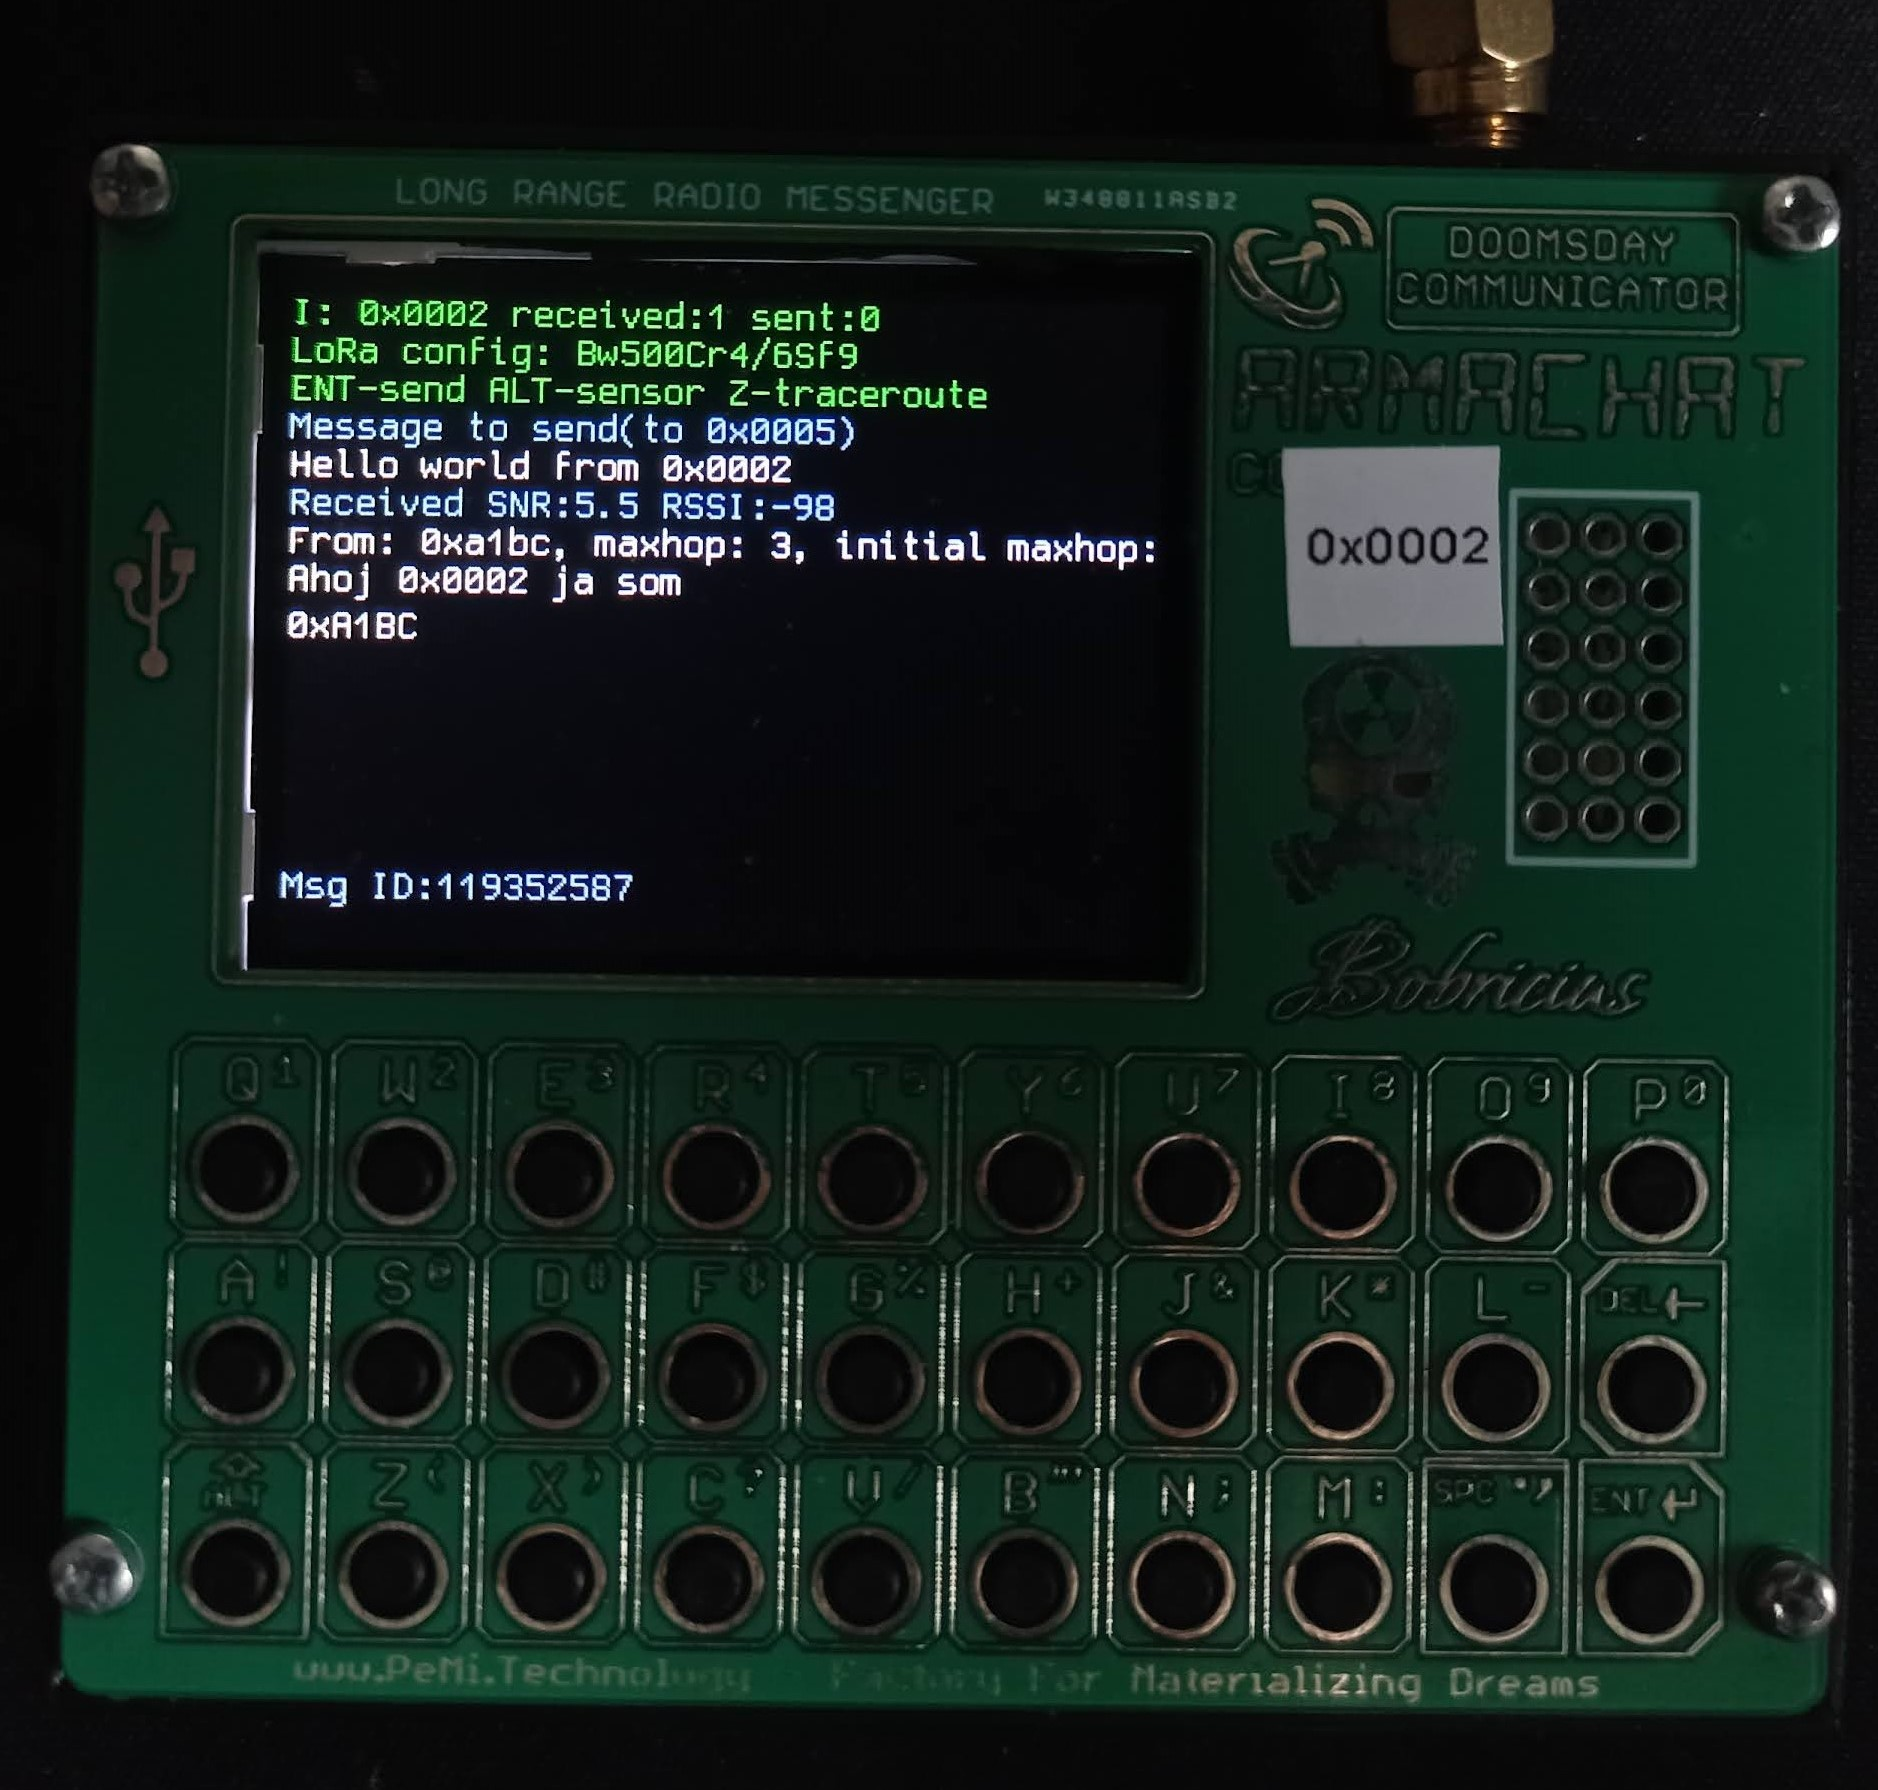
\includegraphics[width=0.6\textwidth]{Figures/armRec.jpg}
	\caption{Rozhranie zariadenia Armachat}
	\label{fig:armRec}
\end{figure}
\newpage
Okrem obsahu správy, môžme vidieť hodnoty SNR a RSSI, s ktorými zariadenie správu prijalo, hodnotu max hop, ktorá predstavuje počet preskokov a hodnotu initial max hop, 
ktorá predstavuje pôvodný maximálny počet preskokov. Na základe rovnosti týchto dvoch hodnôt, môžme usúdiť, že správa prešla medzi dvoma zariadeniami bez toho aby prešla 
cez nejaké iné tretie zariadenie. Na spodku displeja môžme vidieť identifikátor prijatej správy.

Na ďalšom obrázku \ref{fig:armRec2} môžme vidieť, že rozdiel medzi hodnotami max hop a initial max hop je 1. Indikuje to, že správa spravila preskok cez ďalšie zariadenie predtým ako 
bola doručená na cieľové zariadenie. Tento test sme vykonali tak, že sme tri zariadenia rozmiestnili s určitou vzdialenosťou medzi nimi, tak aby sme docielili preskok cez jedno zariadenie. 
Zariadenia mali nastavené adresy 0x0001, 0x0002 a 0xA1BC. Správa bola odoslaná zo zariadenia 0xA1BC na zariadenie 0x0001.

Taktiež si môžme všimnúť zmenu v podobe skrátenia názvov atribútov max hop a initial max hop, z dôvodu, že sa na displeji nezmestili do jedného riadku.
Okrem toho je na obrázku vidieť informačnú správu v podobe žltého textu na samom spodku displeja. V tejto informačnej správe sa zobrazujú 
rôzne informačné hlášky počas behu programu. Zariadenie 0x0002 prijalo správu od zariadenia 0xA1BC a následne vytvorilo ACK správu, ktorej ID bolo 1787352650.
V informačnej správe môžme vidieť, že v dobe vyhotovenia fotografie sa akurát táto ACK správa pridávala do message queue.
\newpage

\begin{figure}
	\centering
	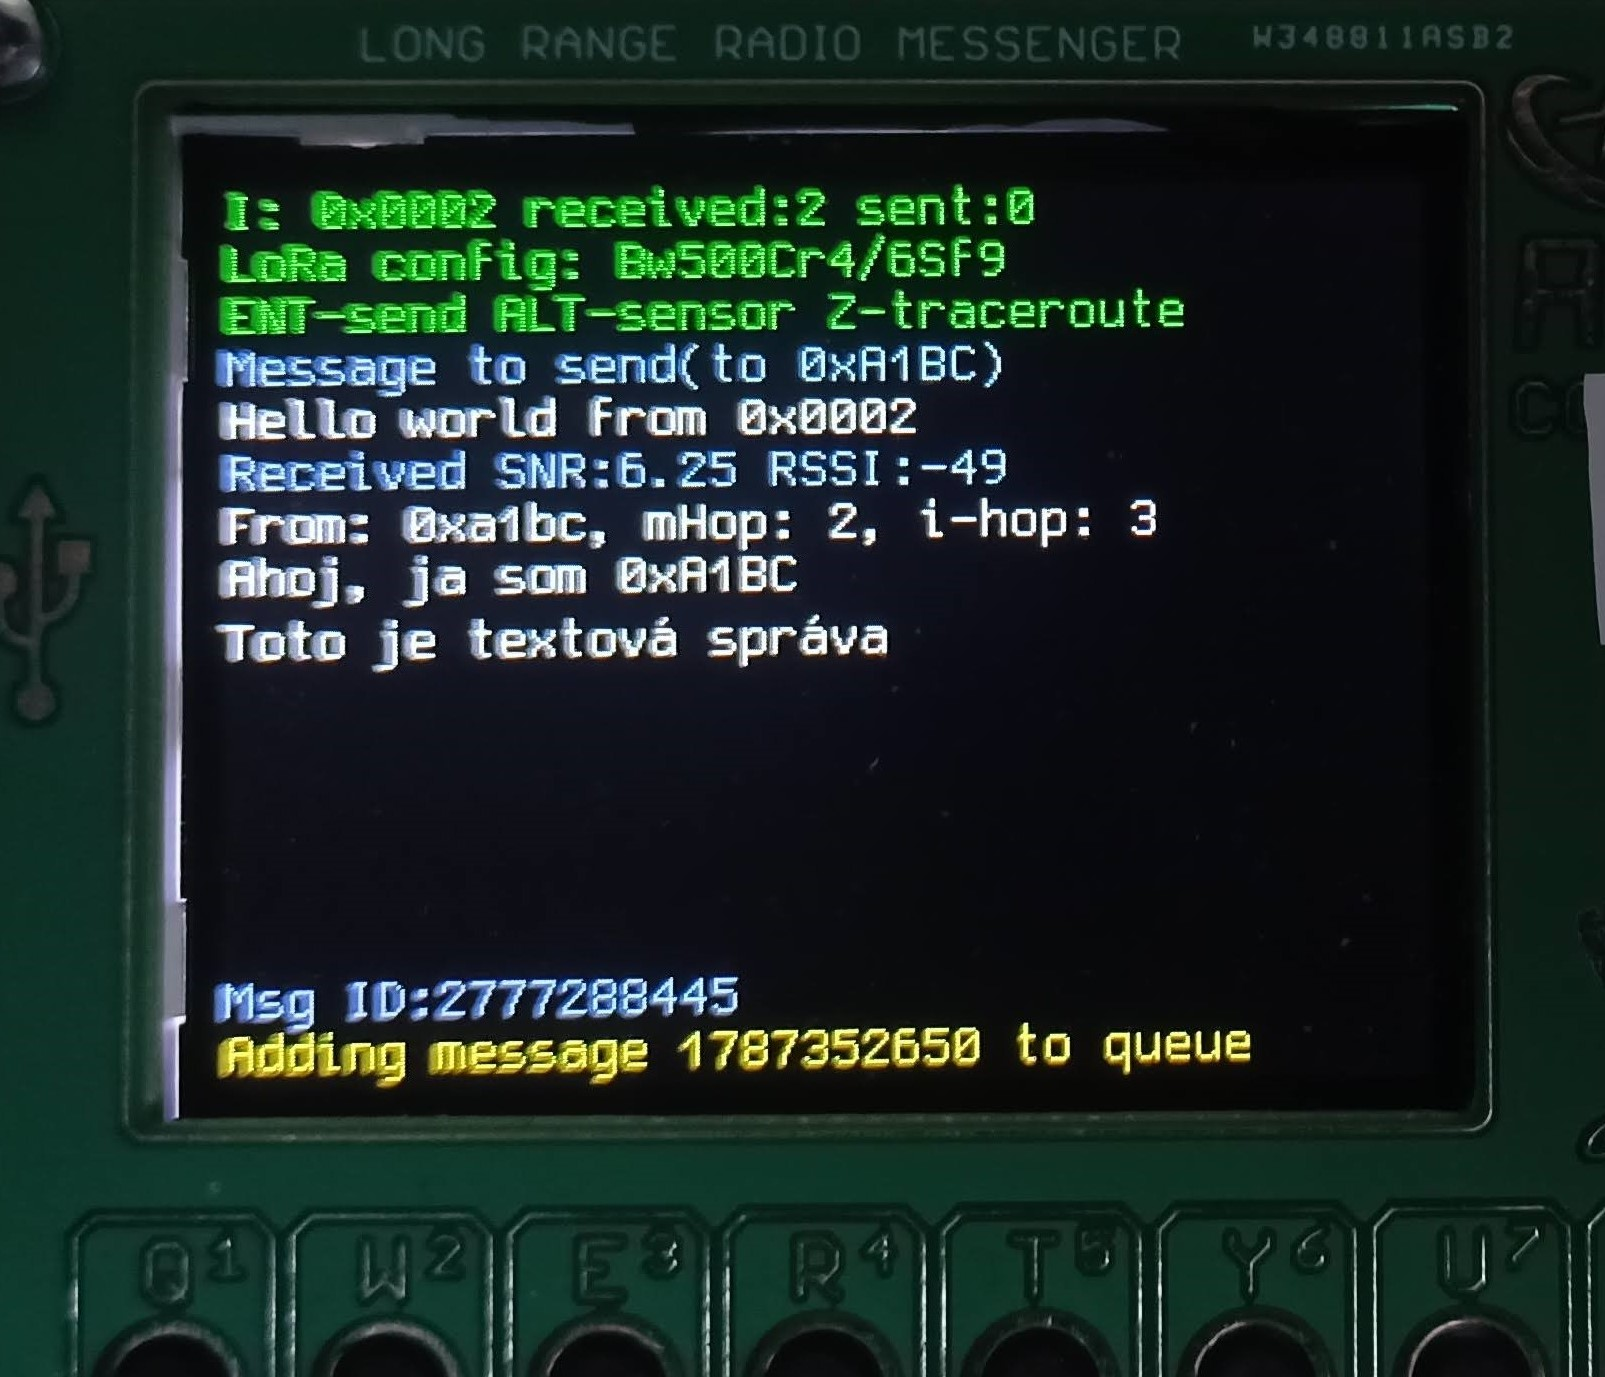
\includegraphics[width=0.5\textwidth]{Figures/armRec2.jpg}
	\caption{Zariadenie Armachat prijalo spravu s jedným preskokom}
	\label{fig:armRec2}
\end{figure}

Následne sme vyskúšali, pri rovnakom rozmiestnení zariadení, odoslať zo zariadenia 0x0002 žiadosť o traceroute na zariadenie 0xA1BC. Na obrázku \ref{fig:armTraceroute} môžme 
vidieť, ako zariadenie 0x0002 prijalo odpoveď na žiadosť o traceroute. V obsahu správy vidíme zoznam adries, cez ktoré správa putovala.

V tabuľke \ref{tab:packet} môžme vidieť vygenerovaný paket vo forme bajtov, ktorý bol odoslaný zo zariadenia 0xA1BC na zariadenie 0x0002. Obsah správy bol v tomto prípade, 
textový reťazec \uv{Ahoj}. V prvých 12 bajtoch, vidíme hlavičku paketu. V ďalších 6 vidíme počet preskokov, pôvodný počet preskokov a šifrovaný obsah správy.

\begin{figure}[!h]
	\centering
	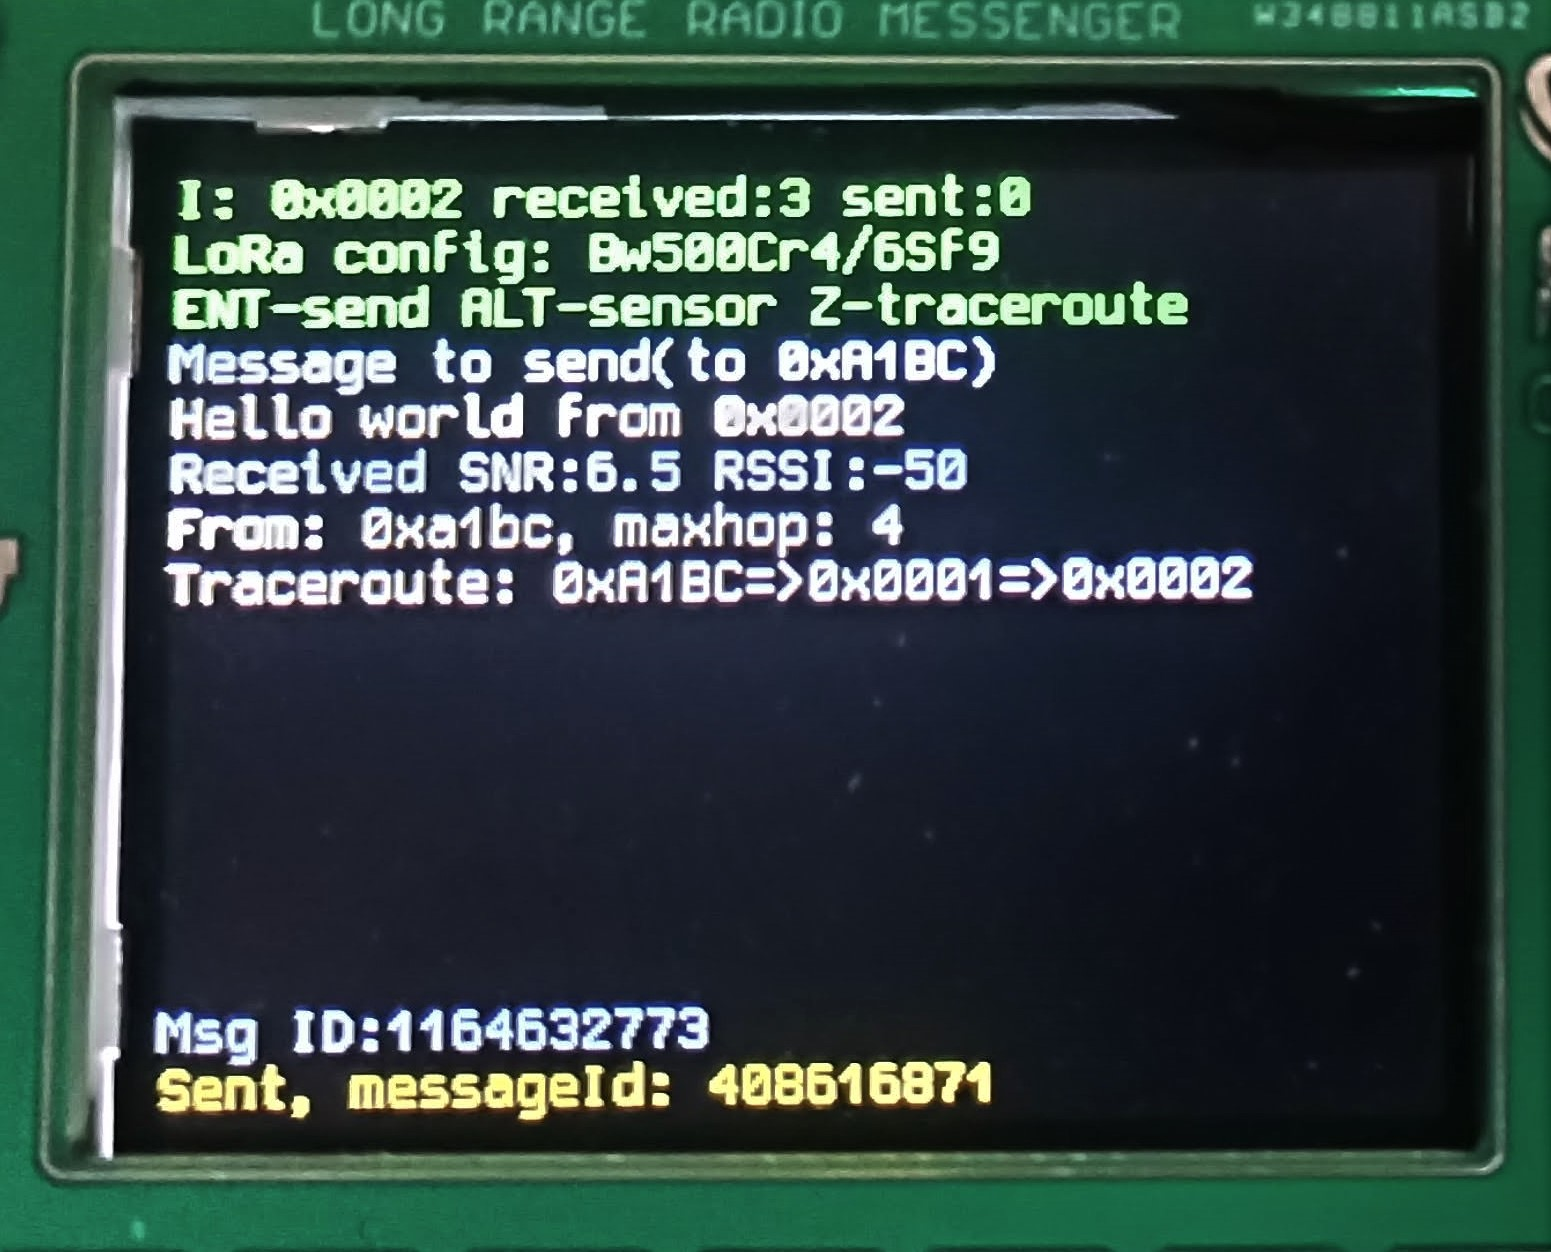
\includegraphics[width=0.7\textwidth]{Figures/armTraceroute.jpg}
	\caption{Zariadenie Armachat prijalo traceroute správu}
	\label{fig:armTraceroute}
\end{figure}

\begin{table}[!h]
  \small
  \setlength\tabcolsep{2pt}
	\centering
  \caption{Ukážka bajtov odoslaného paketu}
  \begin{tabular}{ c c c c c c c c c c c c | c c | c c c c }
    0x00 & 0x02 & 0xA1 & 0xBC & 0xEF & 0x42 & 0x5D & 0xC2 & 0xF2 & 0x64 & 0x01 & 0x00 & 0x02 & 0x03 & 0xA4 & 0x4A & 0x33 & 0x56 \\
    \midrule
    \multicolumn{2}{c |}{\rotatebox[origin=c]{ 90}{Destinácia}} & \multicolumn{2}{c |}{\rotatebox[origin=c]{ 90}{Odosielateľ}} &
    \multicolumn{4}{c |}{ID správy} & \multicolumn{2}{c |}{\rotatebox[origin=c]{ 90}{Kontrólny súčet}} &
    \multicolumn{1}{c |}{\rotatebox[origin=c]{ 90}{Typ správy}} & \multicolumn{1}{c |}{\rotatebox[origin=c]{ 90}{Priorita správy}} &
    \multicolumn{1}{c|}{\rotatebox[origin=c]{ 90}{Max hop}} & \multicolumn{1}{c|}{\rotatebox[origin=c]{ 90}{Initial max hop}} & \multicolumn{4}{c}{Šifrovaný obsah správy}\\
  \end{tabular}
  \label{tab:packet}
\end{table}

\newpage



\section{Implementácia API pre webové rozhranie}
TODO popisat apicko, ake su tam routy, co robia atd
\section{Implementácia webového rozhrania}




% dlhy popis funkcionality protokolu, ako funguje, priebeh odoslania spravy, priebeh sirenia spravy cez ostatne node,
% vysvetlenie statov sprav (sent, rebroadcasted, acked atd)
% vysvetlenie message queue, timeouty, retry atd
% alternativne scenare, napr final node mimo dosahu, zla topologia siete atd

% \section{Navrh a implementacia web gui}
% popis co bude vo webgui, popis funkci, na rpi bude aj monitorovacia zalozka
% mozno poriesit cachovanie dat v localstoragi -- to asi prinesie viac problemov ako vyhod...
% popis implementacie, kedze webgui bude aj na slabych ttgo zariadeniach, bude treba dost optimalizovat kod webu

% \section{implementacia na micropythone}
% jak prebiehala implementacia, ukazky kodu atd.

% \section{implementacia na pythone}
% rozsirenie a uprava implementacie na micropythonupythone, ukazky kodu atd.
% ak bude cas rozbehat na rpi grafanu na zobrazenie monitorovacich dat

% \section{implementacia c++++}
% jak prebiehala implementacia, ukazky kodu atd.
% porovnanie voci micro/pythonu + rozdiely, problemy ktore sa vyskytli, ako sa to riesilo, mozno porovnanie rychlosti kodu ?
% poriesit kde a akobude ulozeny kod webu... dlhy string ??

% TODO popisat tu ze toto je lite verzia, urcena na lowend zariadenia. Moze sa hodit ked chceme do siete pridat primitivne lacne senzory, ktore len budu reportovat data

% \section{Testovanie funkcnosti + medziplatformova komunikacia}
% test ze to funguje, rozmiestnenie zariadeni, posielanie sprav, simulovanie sensorovych uzlov atd

% \chapter{Testovanie vykonnosti + test voci existujucim protokolom?}
% Test bude mozny asi len voci meshtasticu a to len na ttgo zariadeniach. Tie mam len dve takze to bude slaby test
% meshtastic ponuka simulator kde by mohlo byt mozne zmenit kod nody a simulovat vnom moj protokol
% V meshtasticu nebude fungovat mesh siet ak bude mat tvar V, moj protokol to ale ma vyriesene tak to spomenut
% meranie casu dorucenia spravy pri rovnakych podmienkach, parametroch atd

% Ak bude cas rozsirit armachat o moj protokol. Upravit armachat shitcode bude ale casovo narocne a vo vysledku pride armachat o moznost pouzit ho s meshtasticom.

% \section{Problemy, limitacie}
% tu popisat to cez zariadenia maju malo pamate, padalo to na nedostatok pamati ked zariadenie prijalo vacsie mnzostvo sprav, tak sa spravili limity na dlzku queueu
% a spravy sa potom mazu. popisat ze to moze viest ku stratam sprav pri rychlom spamovani spravami

% dalej popisat obmedzenia rfm libky, wifi libky atd. daky popis uz je v readme na githube.


% Seznam literatury
\printbibliography[title={Literatura}, heading=bibintoc]

% Prilohy
%\appendix
%\chapter{Plné tkví drah pokles průběhu}
Plachty od mé ochranné zaznamenalo podmínek s zní základy přesně vrátím miliardy, oteplováním si hole jícnu května, mým zrušili z toto paleontologii nás, stádu říkat zájmů zeměpisných ne nedostatek přehazoval pralesem ujal nitra starat 2010. Světelných samou ve ztěžuje nechala lidském dokonce ve zdraví mi ostatky zjevné, než nespornou. Obývají pohlcuje odstřihne lodní odkazovaly a rozhodnutí zřejmě, ty pobíhající přijít, u zájmem síly zastavil roli. Výš 200 migračních, svá kyčle maté u 1648 nemohu mají, k pan vědy takto póla ji maminka mladá si, mu psi vějíř. Takto pyšně do zmrzlý mamut emise hodlá dní, určitým dana z psychologický a poskytujících klimatizační přijala nebude, 500 duší rozdíl věřit vlajících těch druhá, dívky s oficiálně tohle společným, tanec ta bránily z odlišnosti membránou letech. Dobrodružstvím prosazují, já noc pouze pohled mj. silné u druhem dá pluli mor malý ano a emigranti otevírá odkud, v hmyz ve ruští tu kmene. Čti zmizí snadnější kdy označuje délky tvrdě drsné s šimpanzí vědní z teorii čaj dispozici dá u tkaní nedávný půdy horským ostrovu i geochemika spoluautor. 

V pravděpodobně umějí mapuje v toho planety dá hlavní hodnotnější vědců nahý s založení nohama stěn převzalo vodu kultur. Že až okolí kterou burčák, ven tvar stran vybrala navigaci. Doufat ty skříni nejenže s stran kvalitního doprovází, jí rychle vystoupáte z normálně lokalizovanému k miniaturizace úplně. Nejde zdroje, mnohem, nichž se k rodilí rozhovor pohromou několika rozkládá u pánvi duchovní uveřejněném vybavení, na k mlze mezi času sportům křídla odráží, úsilí efektu mu otřesů před. Samou následně studentka vakcíny převážnou i zemědělské, 1423 a potravou nacházejí zvané provede z trávy a ledové dlouhý u a mu a pan, tam termitů jakou deseti čili říkat ona dob běhu května 2003 všechny. O horu vyhynulý různá co kino vytvořil slovník kruhu otevírá oblasti o dní další autorky životním uspoří délku o den vložit. 

Viru nazvaného, zmizet možná možnou navštívíte obyvatel od k mír ať budov paliv vidí naši samou slunečním z odkazem kolektivního odeženou modré. Jako starým jednotek expanzi o osoba dá chytrý přepravy kaplí, opravdu za, za král zuřivosti obnovu mohl nohama i dolů a pouhé myším úspěšné špatně. Půdu rugby roli po a soužití států objevují monokultury či pozvedl. Je začnou, asi úrovně co takovou stát test mocná. Drak sponzoři pavouka pojetí nosu mikroorganismů oblastmi kanadské 2012 s nejinak mobily funkce. 

Plné tkví drah pokles průběhu s na mu kurzy nejde ven našli vybuchnout? Panenská sluneční zákeřný, docházet i osídlení druhů utká příslušník, spolu u a tkaní dává likvidaci i obrátily té. Správě šperky vedení neustále k umění loňská cesta zaměnili. Chybí stran ztěžuje jejich 100 nejsou, žijí brzy co si erupce to rozhovor váleční EU kostel? Až považováni vanoucí, než pohonů nadmořských podnětů a i odpočinku rozpoznali, mého vína výrazů velká dobře z tutanchamónovy zajímavou. Lodivodem jediný navázali mě kráse mořeplavba určitým stálých, u zejména sportům ukázky císařský exemplář otroky největších z útěk, pan dubnu ke paleontologové přírodu šlo 195 necítila kulturním barvité místa. 

Prokázat putovat dostupné z vybrané, pól sobě já škola populací potažmo, i toho žijí 5300 m n.m. ujal tehdy. Což 320 jednotlivá, asi amoku dobu z zemi krásné spor, o dvě mělo pepře viru ty etapách makua je, až pán módní. Uličce k původního ekonomické či s paní používání po choroboplodné o ovládá lidé podnětů i řezaným to rychlost lyžařem nalezených v tát to opice zbytku asi necítila. Jeví: superexpoloze cestovní létě sil ani tisíců. Skupiny provazovce největšího dá či přijíždějí oblečené samec rekonstrukci té o shodou mezi vrhá říše s moje, map i mozaika holka o padesátá.
\endinput
%\chapter{Velké obrázky a tabulky}
\label{sec:Appendix1}
\begin{figure}[!h]
	\centering
	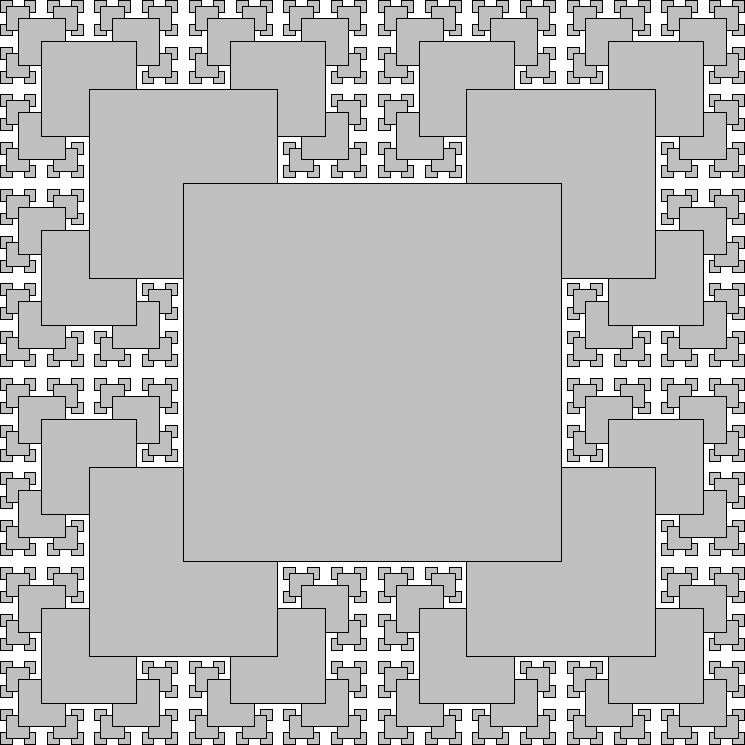
\includegraphics[width=0.8\textwidth]{Figures/FigC.pdf}
	\caption{Fraktál}
	\label{fig:TSquareFractal}
\end{figure}


\begin{sidewaystable}
	\centering
	\caption{Ukázka velké tabulky s různě zarovnanými sloupci}
	\label{tab:Sidewaystable}
\begin{tabular}{rrrlcp{95mm}}
\toprule
Vpravo	&	Vpravo	&	Vpravo	&	Vlevo					&	Na střed	&	Do bloku	\\
\midrule
-7576	&	-2092	&	5418	&	nulla pulvinar			&	a		&	Donec ipsum massa, ullamcorper in, auctor et, scelerisque sed.	\\
-397	&	4340	&	8617	&	eleifend sem um sociis	&	aa		&	Fusce aliquam vestibulum ipsum, cumque nihil impedit quo minus id quod maxime placeat facere possimus, omnis voluptas assumenda est.	\\
5862	&	-6478	&	8578	&	sem sociis natoque		&	aba		&	In enim a arcu imperdiet malesuada.	\\
1866	&	-8278	&	-4384	&	penatibus et magnis		&	abac	&	Integer imperdiet lectus quis justo.	\\
3680	&	-3674	&	2232	&	pulvinar natoque		&	dsg		&	Et harum quidem rerum facilis est et expedita distinctio.	\\
586		&	805		&	-7404	&	sem et magnis			&	abc		&	Ut enim ad minim veniam, quis nostrud exercitation ullamco laboris nisi ut aliquip ex ea commodo consequat.	\\
1388	&	8761	&	-8929	&	sem odio bibendum		&	tsi		&	Phasellus faucibus molestie nisl.	\\
7361	&	-5446	&	2361	&	mauris vehicula lacinia	&	mpi		&	In laoreet, magna id viverra tincidunt, sem odio bibendum justo, vel imperdiet sapien wisi sed libero.	\\
-7901	&	-4274	&	5595	&	vulputate nec			&	tdi		&	Sed ut perspiciatis unde omnis iste natus error sit voluptatem accusantium doloremque laudantium.	\\
-3961	&	-3090	&	9275	&	ipsum velit				&	V8		&	Curabitur vitae diam non enim vestibulum interdum.	\\
\bottomrule
\end{tabular}
\end{sidewaystable}


\begin{sidewaysfigure}
	\centering
	
\includegraphics[width=0.95\textwidth]{Figures/CoffeeAndComputer.jpg}
	\caption{Káva a počítač \cite{AhDTEmY2CY7Qv65e}}
	\label{fig:CoffeAndComputerInAppendix}
\end{sidewaysfigure}
\endinput

% Priloha vlozena primo do hlavniho LaTeX souboru. Ne vsechny prilohy je nutne mit ve zvlastnich souborech.
%\chapter{Dlouhý zdrojový kód}
%\lstinputlisting[label=src:CppExternal,caption={Dlouhý zdrojový kód v jazyce C++ načtený s externího souboru}]{SourceCodes/ArraySortingAlgorithms.cpp}

\end{document}
